\documentclass[12pt,a4paper,twoside,openright]{book}

\usepackage[dvips]{graphicx}
\usepackage{tabularx}
% \usepackage{subfigure}
\usepackage{subcaption}
\usepackage{afterpage}
\usepackage{amsmath,amssymb}            
\usepackage{rotating}  
\usepackage{fancyhdr}  
\usepackage{caption}%[scriptsize]%
\usepackage[T1]{fontenc}
\usepackage[utf8]{inputenc}
\usepackage[italian, british]{babel}
\usepackage{times}
\usepackage{graphicx}
\usepackage{listings}
\usepackage{color}
\usepackage{microtype}
\usepackage{url}
\usepackage{float}
\usepackage{tabularx,ragged2e}
\usepackage{pgfplots}
\pgfplotsset{compat=1.9}
\newcolumntype{x}{>{\Centering}X}


\definecolor{dkgreen}{rgb}{0,0.6,0}
\definecolor{gray}{rgb}{0.5,0.5,0.5}
\definecolor{mauve}{rgb}{0.58,0,0.82}

\lstset{
frame=tb,
  language=Java,
  aboveskip=3mm,
  belowskip=3mm,
  showstringspaces=false,
  columns=flexible,
  basicstyle={\small\ttfamily},
  numbers=none,
  numberstyle=\tiny\color{gray},
  keywordstyle=\color{blue},
  commentstyle=\color{dkgreen},
  stringstyle=\color{mauve},
  breaklines=true,
  breakatwhitespace=true,
  tabsize=3
}

\lstset{
    breaklines=true,
    basicstyle=\ttfamily\scriptsize,
    numbers=left,
    postbreak=\raisebox{0ex}[0ex][0ex]{\ensuremath{\space}}  
}

\usepackage{xspace}
\usepackage{indentfirst}
\usepackage{todonotes}

\setlength{\paperwidth}{16cm}
\setlength{\paperheight}{24cm}
\setlength{\oddsidemargin} {2. cm}
\setlength{\evensidemargin} {2. cm}
\addtolength{\oddsidemargin} {-0.4 cm}
\addtolength{\evensidemargin} {-0.4 cm}
\linespread{1.15}

\renewcommand{\captionfont}{\normalfont \sffamily \itshape \small}


\newcommand{\eg}{\textit{e.g.,}\xspace}
\newcommand{\ie}{\textit{i.e.,}\xspace}

\graphicspath{{pictures/}}

\begin{document}

\frontmatter
\pagenumbering{Roman}

\title{Tesi}
\thispagestyle{empty}
%\begin{titlepage}
\vspace*{-1.5cm} \bfseries{
\begin{center}
  \large
  POLITECNICO DI MILANO\\
  \normalsize
  Scuola di Ingegneria Industriale e dell'Informazione
  \\
  Corso di Laurea Magistrale in Ingegneria Informatica
  \\
  Dipartimento di Elettronica Informazione e Bioingegneria
  \\
  \vspace{5mm}
  \begin{figure}[htbp]
    \begin{center}
    
\includegraphics[width=3.5cm]{pictures/logopm.png}
%       
\includegraphics[width=3.5cm]{./pictures/logopm}
%	
\psfig{file=./pictures/logopm.jpg,width=3.5cm}
    \end{center}
  \end{figure}
  \vspace*{0.3cm} \LARGE



  \textbf{Programming Abstractions for Nano-drones Teams}\\



  \vspace*{.75truecm} \large
\end{center}
\vspace*{3.0cm} \large
\begin{flushleft}


  Relatore: Prof. Luca Mottola \\
  Correlatore:  Mikhail Afanasov\\


\end{flushleft}
\vspace*{1.0cm}
\begin{flushright}


  Tesi di Laurea di:\\ Manuel Belgioioso, matricola 804149 \\ 
		       Alberto Cardellini, matricola 818246  \\


\end{flushright}
\vspace*{0.5cm}
\begin{center}



  Anno Accademico 2014-2015
\end{center} \clearpage
}\thispagestyle{empty} \normalfont 
\cleardoublepage

\linespread{1.20}
\pagestyle{plain}
\vspace{17cm}

\begin{flushright}
\itshape{Alle nostre famiglie.}
\end{flushright}
\chapter*{Abstract}

\addcontentsline{toc}{chapter}{Abstract}

% VERSIONE CARDE 
Drone-teams programming is rapidly expanding since it allows to automatically perform a lot of useful tasks.
Existing systems are able to manage a group of drones and dispatching them in the environment. 
All these systems deal with outdoor applications, where medium/big sized drones collaboratively perform tasks making use of the Global Positioning System (GPS) to navigate in the space.
Our goal is to fill a gap in the available programming models so that it could be possible to develop a drone application with the concept of Trip. A Trip can be considered as a movement from a source point to a destination.
Furthermore the second important goal is making the system autonomous while choosing the drone to allocate for each Trips. This means that the user does not need to take this important decision.
We focused our efforts in the creation of an indoor capable programming framework, this means dealing with many implementation challenges.
From a technological point of view, GPS cannot be used in indoor contexts, so we need to find an appropriate indoor localization method.
Then indoor contexts imply small areas which are usually full of people and/or obstacles (think of an house context) hence, drones have to be small, in order to avoid crashes.
Size limitations result in many problems such as the battery autonomy and the maximum weight transportable.
We propose the Pluto programming framework as a solution to these problems. It consists in two main components: the Graphical Editor and the Main Application. With the former a programmer can build an application by simply connecting blocks.
Each block implements a precise functionality, for example there is one that choose the drones for the sensing tasks, one that manages the priority of each sensing tasks etc.
Then the developer can generate the source code  of the second main component of Pluto, from the built graph. The final user will use this generated Pluto Main Application to specify and execute the sensing tasks.
We fully evaluated the Pluto programming framework by proposing its use to real testers and asking them for a feedback. Moreover we measured its software and hardware performances and also tried to implement some existing applications with it.
After the evaluation we noticed that, even if with some limits, Pluto could be useful to simplify the developing of drone-teams applications.



% ----------------------- PARTE VECCHIA --------------------------------
% Drone-teams programming is rapidly expanding since it allows to automatically perform a lot of useful tasks.
% Existing systems are able to manage a group of drones, dispatching them in the environment. 
% All these systems deal with outdoor applications, where medium/big sized drones collaboratively perform tasks making use of the Global Positioning System (GPS) to navigate in the space.
% We want to develop a team-level programming framework for indoor applications.
% Dealing with an indoor context means dealing with many limitations, both in the system implementation and in the technologies to be used.
% From a technological point of view, GPS cannot be used in indoor contexts, so we had to find an indoor localization method.
% Indoor contexts imply small areas which are usually full of people and obstacles (think of an house context) hence, drones have to be small, in order to avoid crashes with both human and environmental obstacles.
% Size limitations result in many problems; the first is battery duration, which can reach a maximum of 10 minutes, having a recharge time of about 20/30 minutes.
% From an implementation point of view, no one of the existing systems deals with a \textit{Trip} concept, that is nothing but a movement from a point A to a point B in the environment to perform an \textit{Action}.
% We took into account all these problems and found a solution to them and finally we developed the Pluto programming framework.
% Pluto has two components: the Graphical Editor and the Main Application.
% With the former a programmer can build an application by simply connecting blocks.
% Each block implements a precise functionality, for example there is one that assign the drones to the sensing tasks, one that manage the priority of each sensing task etc.
% Then the programmer can generate the code from the built graph and the final user can use the Pluto Main Application to decide the sensing tasks to be performed.
% We fully evaluated the Pluto programming framework by proposing its use to real testers and asking them for a feedback, measuring its software and hardware performances and also trying to build existing applications with it.
% After the evaluation we noticed that, even if it has some limits, Pluto is a useful programming framework that can be used to develop a lot of drone-teams applications.



\begin{otherlanguage*}{italian}
\chapter*{Sommario}

\addcontentsline{toc}{chapter}{Sommario}

I droni autonomi stanno compiendo una vera e propria rivoluzione nel campo del rilevamento mobile:
vari tipi di droni sono utilizzati per eseguire un gran numero di applicazioni, in quanto possono trasportare una gran quantità di dati raccolti grazie a sensori quali fotocamere e microfoni.
Spesso vi è una semplice astrazione che permette ai droni di navigare nell'ambiente: possono essere controllati tramite interfacce grafiche per smartphone e tablet o impostando dei waypoint.
I droni possono notevolmente estendere le capacità dei sistemi di rilevamento tradizionali riducendo al contempo i costi.
Si possono monitorare le colture di un agricoltore, gestire i parcheggi, o monitorare i sistemi di telecomunicazione sottomarini in maniera più pratica e/o più a buon mercato rispetto ai sensori fissi.
La grande innovazione portata dai droni è che offrono un controllo diretto sui punti da monitorare  nell'ambiente; questo era impossibile con i precedenti sistemi di rilevamento mobili che potevano solo passivamente rilevare l'ambiente, basandosi sulla mobilità di smartphone o veicoli.
Così, i droni possono estendere notevolmente il campo del rilevamento mobile, permettendo ai programmatori di creare un gran numero di applicazioni, impensabili precedentemente e impossibili da sviluppare con le tecnologie già esistenti.
\end{otherlanguage*}
\chapter*{Acknowledgements}

\addcontentsline{toc}{chapter}{Acknowledgements}

\noindent
It is a pleasure to thank those who made this thesis possible with advices, critics and observations.

\noindent
We would like to thank our supervisor Prof. Luca Mottola and our mentor Mikhail Afanasov: without their help and support, this thesis would not have been possible.\\

\noindent
We would like to thank Prof. Thiemo Voigt, who kindly let us developing part of this work at SICS Swedish ICT and all the colleagues who have greeted and helped us during the three months in Sweden, in particular Simon Duquennoy, Liam McNamara and Nicklas...\\

\noindent
We owe our deepest gratitude to our families and friends for the continuous support during these years at university.\\

\noindent
Finally, we would like to thank one with the other for having lived together this experience.\\
\tableofcontents
\listoffigures

\pagestyle{plain}\renewcommand{\chaptermark}[1]{\markboth{\chaptername\ \thechapter.\ #1}{}} 
\renewcommand{\sectionmark}[1]{\markright{\thesection.\ #1}}         
\fancyhead[LE,RO]{\bfseries\thepage}    
                                        
\fancyhead[RE]{\bfseries\leftmark}    
\fancyhead[LO]{\bfseries\rightmark}     
\renewcommand{\headrulewidth}{0.3pt}

\mainmatter
\chapter{Introduction}
\label{cap1}

Autonomous drones are performing a revolution in the field of mobile sensing: various type of drones are used to perform a great number of applications, since they can carry rich sensor payloads, such as cameras and instruments.
Often there is a simple abstraction which allows drones navigation: they can be controlled through mobile devices or by setting waypoints from a desktop application.
The great deal with drones is that they can greatly extend the capabilities of traditional sensing systems while simultaneously reducing cost.
\\

Many drones applications have been developed in the recent years, performing a wide range of different functionality, but they are all suitable for outdoor contexts.
We aim to create a new programming model for the collaboration of nano-drones, in order to extend the support for the developers who want to create new applications in indoor contexts.
\\

The indoor context implies applications with different requirements compared to the outdoor ones:
there is need for a small number of drones(5/10), each one performing a different action independently from the others, while in the outdoor environment generally there is need for a large number of drones to perform the same action.
We formalize this problem with the concept of \textit{Trip}, that is nothing but a movement of a drone from a point A to a point B at the end of which an action (picture,measurement etc.) is performed.
Existing frameworks do not allow the developer to deal with the concept of Trip.
We also want to make our framework autonomous while choosing which drone has to physically carry out the Trip.
\\

From a technological point of view, GPS cannot be used in indoor contexts.
Furthermore, the indoor context implies moving in small areas which are usually full of people and obstacles, so the drones have to be small, in order to avoid crashes with both human and environmental obstacles.
Size limitations result in other problems such as the low battery duration and the maximum transportable weight.
So, we need to give a contribution to the actual state of the art in order to derive a new programming system crossing all the previous requirements.
Our programming framework has an architecture in which the central brain is independent from the particular navigation API, which means that the system manages the dispatching of drones and their failures independently of the specific navigation algorithm.


\section{Contribution}

Imagine a medical context where the nurses' duty is to deliver, every day at the same hour, the patients' daily medicines.
A drone could achieve this task flying room by room and leaving the pills to the relative patient's desk. 
It would be way better if a group of drones could manage these tasks simultaneously.
\\

In order to create an application able to carry out this task, a developer could program each drone individually, making use of a specific API to command them, and taking care of the complex duty of managing the coordination between them. 
Our goal is to build a more clever programming framework, where a central brain manages the dispatching of the drones simultaneously and expresses how the drones should behave to accomplish these tasks, managing also the failures due to crashes of the drones and batteries getting empty. 
Chapter \ref{cap2} illustrates in details the possible ways to achieve this goal:
instead of using a \textit{Drone Oriented} approach, the developer could use either a \textit{Swam Oriented} or a \textit{Team Level} approach. 
There are several available frameworks such as Karma\cite{karma} and Voltron\cite{voltron}, but no one of them is fully suitable for our programming model, shown in section \ref{programmingModel}.
\\

As already said, we deal with the indoor context, that implies applications with different requirements compared to the outdoor ones:
there is need for a small number of drones(5/10), each one performing a different action independently from the others, while in the outdoor environment generally there is need for a large number of drones to perform the same action.
We formalize this problem with the concept of \textit{Trip}, that is nothing but a movement of a drone from a point A to a point B at the end of which an action (picture,measurement etc.) is performed. 
No other framework allows the user to define the idea of a Trip as a movement from point A to point B to accomplish an action.
Another fundamental feature of our framework is that the central brain takes care of the important decision to choose which drone to assign to a given Trip, facilitating the work of the programmer in the development of his application.
As said, the system manages the failed trips in the same way.
For example, when a drone crashes, the system chooses a new drone to complete the interrupted Trip, without any intervention of the programmer and the final user.
\\

We wanted to facilitate as much as possible the work of the programmer, so we decided to create the Graphical Editor, fully described in Section \ref{plutoGraphicalEditor}.
Thanks to this editor, the programmer can develop its application by drawing functional blocks and then connecting them with arrows.
Each block represents a feature: there is a block that assigns a Drone to a Trip, one that sends the drones to the target location, etc.
The developer can connect the blocks needed according to the requirements of the specific application.
From the drawn graph the programmer can generate the source code of the Main Application mentioned before. This source code is dependent on the graph and adds to the Main Application all the features expressed by the chosen blocks.
\\

In order to define the sensing tasks, we developed the Pluto Main Application, that is the final user interface fully described in Section \ref{plutoMainApp}.
It allows the final user to choose the actions to perform and where they must be performed, by simply dragging and dropping the actions on a map. 
An Action could be the taking of a photo, a measurement of some parameters or a custom task expressed by the developer.
\\

Finally we evaluated the Pluto framework under different points of view, as described in Chapter \ref{cap6}. 
First of all, we chose some already existing applications and tried to develop them from scratch with Pluto.
Then we evaluated the framework usability, proposing some exercises to real testers and asking them for a feedback through a survey.
Finally we focused our attention on the software and hardware metrics such as the code complexity and the CPU consumption. 
We defined some metrics to evaluate both the users' exercises and the software and hardware metrics.
After a detailed analysis of both the metrics results and the answers to the user survey,
the results convinced us about Pluto capability to simplify the duties of a developer in implementing a drone application.
The whole evaluation process is shown in Chapter \ref{cap6}


\section{Outline}

In this Chapter, we have given the general context and the general goals of the work together with a brief description of our work.
\\

In Chapter~\ref{cap2} there is a description of the actual state of the art in the context of our work.
In Sections \ref{droneLevel}, \ref{swarmLevel} and \ref{teamlevel} we describe the three main existing approaches for drone programming, the "Swarm-level","Drone-level" and "Team-level" respectively, also proposing existing examples for each one of them.
We show that no one of these approaches is suitable for our requirements, since we need the concepts of missions and trips.
A mission is a list of sensing tasks to be performed sequentially and a trip is a movement from a point A to a point B in the environment to perform an action.
Then, in Section \ref{dataflow}, we describe the dataflow programming method, that we adopted for the Pluto Graphical Editor, providing two existing examples of it.
Also in this case, we show that we need a different approach, since we need to use only a group of basic components for our work, while the existing solutions are too general and include a lot of complex components.
\\

Chapter~\ref{cap3} is focused on the problems stemming from the indoor context and on the requirements deriving from it.
In Section \ref{motivating}, we show a motivating example application, in order to better explain the requirements and problems deriving from our work.
In Section \ref{teamlevelproblems} we show the implementation problems deriving from using a Team-level approach for our system, also proposing the solutions to fix them.
Finally, in Section \ref{challenges} we show the technological limitations affecting our system, such as the indoor localization and nano-drone batteries problems.
\\

Chapter~\ref{cap4} presents our solution for the research problems described in Chapter ~\ref{cap3}, the Pluto programming framework.
In Section \ref{programmingModel} we present our programming model:
we show the entities of our model and the relationships between them.
We also describe the blocks architecture of the Pluto Programming Framework, which is shown in Section \ref{functionalBlocks}.
In Section \ref{functionalBlocks} we describe in details the functionality of the available blocks of the Pluto Graphical Editor, that are the basic elements that the programmer can connect to graphically build an application.
In Section \ref{toolchain} we describe in details the two components of the Pluto framework:
the Graphical Editor, that is used by the programmer to graphically build an application and the Main Application, that is used by the final user to specify the sensing tasks to be performed.
In Section \ref{navigationSystem} we describe the navigation system, that is the conjunction point between the Main Application and the drones team.
The last Section of the Chapter, the \ref{history}, describes all the steps performed to arrive to the final system, showing all the previously implemented solutions which, once refined, brought us to the development of the Pluto programming framework.
\\

Chapter~\ref{cap5} shows how the designed choices have been implemented technically, describing all the software and tools used for the development of Pluto programming framework.
In Section \ref{editor} we describe the GEF framework, which we used to implement the Pluto Graphical Editor.
In Section \ref{codeGeneration} we show the code generation process that creates a Java application from the graph built with the Pluto Graphical Editor.
In Section \ref{oomodel} we motivate the choice of an Object-Oriented programming model for the Pluto framework.
In Section \ref{runtimeMng} we describe the runtime features of Pluto:
the parallel architecture and the management of all the needed threads.
In Section \ref{interface} we describe the SWING tool, which we used to develop the Pluto Main Application.
Finally, in Section \ref{crazyflie} we describe the Crazyflie nano-quadcopter, which we used to perform the sensing tasks of our prototype applications.
\\

Chapter~\ref{cap6} starts with an analysis on the applicability of the Pluto framework.
In Section \ref{applicability} we describe four already existing applications and three case study, and we discuss on whether they can be developed or not with Pluto. 
In Section \ref{usability} we propose two exercises to real testers, in order to test "on the field" the effective usability of Pluto:
the first one deals with the Graphical Editor, the second one with the Main Application.
Then we propose a third exercise, in which we ask the users to directly use the API of the Crazyflie nano-quadcopter, shown in section \ref{crazyflie}, to make it move from a point A to a point B.
We also propose a survey to the users and then present the result in a graphical way, in order to have opinions on the framework and possibly to improve it with the suggestions of the testers.
In Section \ref{performance} we measure the software and hardware consumption metrics required by Pluto, in order to evaluate the effective impact of Pluto on an ordinary computing machine.
\\

Finally, Chapter~\ref{cap7} draws the conclusion and recaps the results obtained, also showing the possibilities for future works to extend our programming model.
\chapter{State of the art}
\label{cap2}

In the last years, the drone technology is expanding rapidly;especially the aerial drones, which are often used as toys controlled by joystick  or to make aerial videos through mounted cameras.
There exist also aquatic and terrestrial drones, which can be used for many applications. 
For example, through aquatic drones the submarine network infrastructure\cite{submarine} could be managed more efficiently, and through terrestrial drones some emergency situations, like fires, can be managed without involving human life.

Basically, the mobile sensing through drones represents a technological revolution, opening the way for many applications which could not have been developed with the traditional technologies.
Actually, there are a lot of fields where this new technology could be applied, improving performance and reducing costs:
for example surveillance applications, instructing drones to fly over an area monitoring people, or an application in a domestic context, for example instructing drones to find a lost object or to perform some kind of actions, like bringing some objects to the final user.

In the following Section we present three main approaches for programming drones , providing existing examples for each one of them:

\begin{itemize}
\itemsep2pt
\item{
\textit{Drone-level approach}, described in Section \ref{droneLevel}
}
\item{
\textit{Swarm-level approach}, described in Section \ref{swarmLevel}
}
\item{
\textit{Team-level approach}, described in Section \ref{teamlevel}
}
\end{itemize}

The former is focused on the programming of an every single drone, while the second implies basic rules to execute for the whole swarm of drones. The third approach is the most modern work. It creates a middle-ground between drone and swarm approaches, by providing a flexibility in expressing sophisticated collaborative tasks without addressing to a single drone.

After presenting the three main approaches for programming drones, we show some examples of data-flow

\section {Drone-level approach}\label{droneLevel}

In the Drone-level approach, the programmer must manage the single drone, taking care of giving a list of instructions that the drone will perform sequentially.
This approach may be suitable for applications where there is a single drone performing some actions, like searching for a lost object and bringing it back to the user.But scaling the application to a number of drones makes programmer to deal with  concurrency and parallelism. Moreover, battery and crashes/failures should be managed manually for every drone. Finally, timing constraints and a dynamic load balance drastically increase the complexity of the programming. For these reasons drone-level approach is not suitable for a large number of drones.
\\

A concrete example of the application of the Drone-level approach is the so called Robot Create(fig.~\ref{fig:irobot}), a hobbyist robot manufactured by iRobot\cite{irobot} that was introduced in 2007 and based on their Roomba vacuum cleaning platform. The iRobot Create is explicitly designed for robotics development and improves the experience beyond simply hacking the Roomba. 
Since the built-in serial port supports the transmission of sensor data and can receive actuation commands, any embedded computer that supports serial communication can be used as the control system.
\\

To control the Create, the developer should send a sequence of commands through the serial interface. Each command starts with a one-byte opcode and some of them must be followed by data bytes. For example to control the wheel actuators the developer should send a command like this:
\\

\textit{[137] [Velocity high byte] [Velocity low byte] [Radius high byte] [Radius low byte]}
\\

It takes four data bytes, interpreted as two 16-bit signed values using two’s complement. The first two bytes specify the average velocity of the drive wheels in millimeters per second (mm/s), with the high byte being sent first. The next two bytes specify the radius in millimeters at which Create will turn.
\\

\begin{figure}[H]
  \centering
  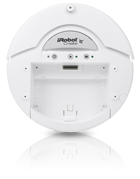
\includegraphics[width=5cm,height=5cm]{pictures/Irobot.png}
  \caption{The iRobot Create}
  \label{fig:irobot}
\end{figure}

A number of robot interface server / simulators support the iRobot Create. Most notably, the Player Project has long included a device interface for the Roomba, and developed a Create interface in Player 2.1. The Universal Real-time Behavior Interface (URBI) environment also contains a Create interface.
This robot is designed for a single execution of a single task without being connected with other robots. Moreover, the design does not imply the collaboration with other robots.
\\

\section{Swarm-level approach}\label{swarmLevel}

The Swarm-level approach\cite{swarm} is more suitable for applications where a number of drones are supposed to perform the same actions. Indeed the programmer can give a set of basic rules that each drone in the swarm can follow.
It is important to underline that, in swarm-level approach, there is no possibility to have a shared state between drones; each drone execute the actions specified by the programmer on his own local state.
It enables the scaling of the approach, but it's not suitable for applications that require the drones to explicitly coordinate.
For example, the swarm-level approach could be applied in an application where many drones take objects at different locations and bring them to the final user, without considering any time or space coordination between them; each drone will simply bring the object back to the user when found.  
There are several existing applications using the swarm-level approach, but we decided to describe three of them:
the Robot Operating System (ROS)\cite{ros}, which provides a Publish/Subscribe coordination layer for decentralized computations, as shown in Section \ref{ros}; Karma\cite{karma}, which lets programmers specify modes of operation for the swarm, such as “Monitor” or “Pollinate”(as shown in Section \ref{karma}); and Proto\cite{proto}, which lets programmers specify actions in space and time(as shown in Section \ref{proto}). 

\subsection{Robot Operating System}\label{ros}

ROS\cite{ros} is not an operating system in the traditional sense, indeed it provides a layer for communication between many, possibly heterogeneous, operating systems connected in a cluster.

The whole functioning of ROS, shown in fig.\ref{fig:ros}, is based on \textit{Nodes}, which are software modules performing computations; the whole system is composed by many nodes exchanging messages, according to the \textit{Publish-Subscribe} model:
a node can send messages publishing them on a particular \textit{Topic}, and nodes which are interested in a particular topic simply subscribe to it; publishers and subscribers don't know each others' existence.
The publish-subscribe topic based communication model is very flexible, but is not suitable for synchronous exchanges, because of its broadcast functioning; for this reasons ROS provides also \textit{Services}, which are composed by a name and two messages, one for the request and one for the response.

\begin{figure}[htbp]
  \centering
  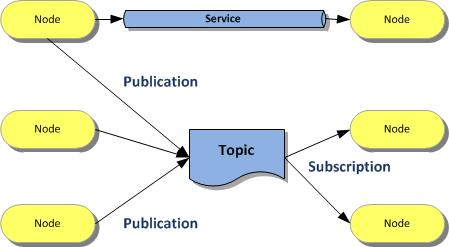
\includegraphics[width=\linewidth]{pictures/ros.jpg}
  \caption{ROS communication layer functioning}
  \label{fig:ros}
\end{figure}


\newpage

\subsection{Karma}\label{karma}

Karma\cite{karma} is a resource management system for drones swarms based on the so called hive-drone model; the hive-drone model is a feature that moves the coordination complexity of the application to a centralized computer: the hive is the base station where drones can land, if they are not busy, and charge their batteries; the hive also takes care of dispatching the drones in order to perform the actions specified by the programmer to accomplish the swarm objectives; the programmer specifies the desired swarm behaviour through a programming model which allows him not to deal with a coordination between drones.

The Karma\cite{karma} runtime at the hive is composed by functional blocks, as shown in fig.~\ref{fig:karma}:

\begin{itemize}
\itemsep2pt
\item{
\textit{Controller}: is the overall manager of the runtime and invokes the other modules when needed; when a user submits an application to the Karma system, the hive Controller determines the set of active processes, and invokes the Scheduler to allocate the available drones to them.
}
\item{
\textit{Scheduler}: is periodically invoked by the Controller to allocate drones to each active process.
}
\item{
\textit{Dispatcher}:  is responsible for tracking the status of the drones; it programs the drones with the allocated behavior prior to a sortie, tracks the size of the swarm, and notifies the Controller when a drone returns to the hive and is ready for redeployment.
}
\item{
\textit{Datastore}: when drones return to the hive, they transfer the data they collected to the Datastore.
}
\end{itemize}


\begin{figure}[htbp]
  \centering
  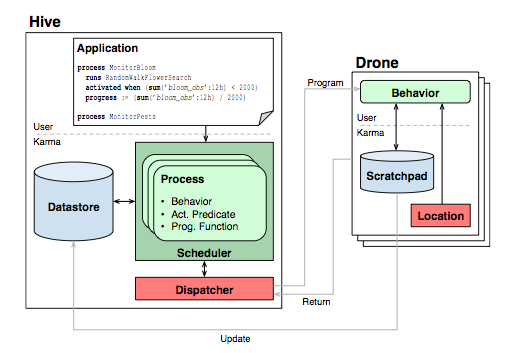
\includegraphics[width=\linewidth]{pictures/Karma.png}
  \caption{The basic schema of Karma}
  \label{fig:karma}
\end{figure}

\newpage

\subsection{Proto}\label{proto}

The amorphous medium abstraction\cite{medium} is derived from the observation that in many spatial computing applications, we are not interested in the particular devices that make up our network, but rather in the space through which they are distributed; indeed, for example, the only things that matter for a sensor network are the values that it senses, not the particular devices it's composed of.
The amorphous medium\cite{medium} takes this concept to the extreme: indeed it is defined as a spatial area with a computational device at every point, as shown in fig.\ref{fig:medium}: Information propagates through this medium at a maximum velocity. Each device is associated with a neighborhood of nearby devices, and knows the "state" of every device in its neighborhood, i.e. the most recent information that can have arrived from its neighbors.



\begin{figure}[H]
  \centering
  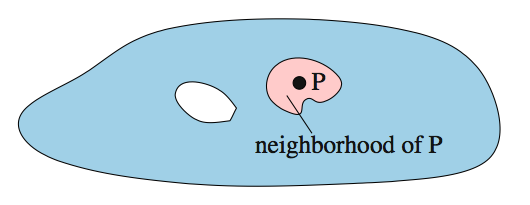
\includegraphics[width=\linewidth]{pictures/ProtoMedium.png}
  \caption{The amorphous medium abstraction}
  \label{fig:medium}
\end{figure}



The Proto\cite{proto} language uses the amorphous medium abstraction\cite{medium} to divide the spatial programming problem in three sub-problems, as shown in fig.~\ref{fig:proto}:

\begin{itemize}
\itemsep2pt
\item{
global descriptions of programs as functional operations on fields of values
}
\item{
compilation from global to local execution on an amorphous medium
}
\item{
discrete approximation of an amorphous medium by a real network
}
\end{itemize}


\begin{figure}[h!]
  \centering
  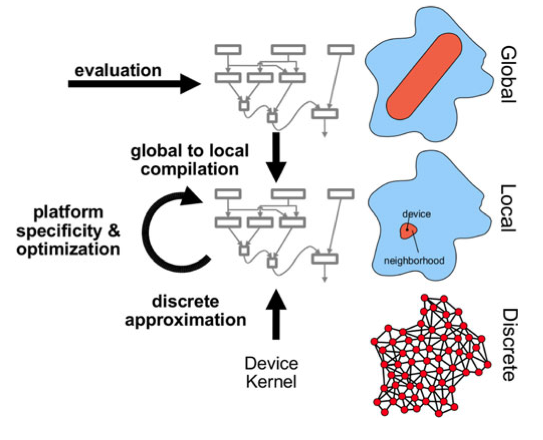
\includegraphics[width=\linewidth]{pictures/Proto.png}
  \caption{Proto: problem decomposition}
  \label{fig:proto}
\end{figure}

To apply Proto\cite{proto} language to mobile devices, such as drones in a swarm, the amorphous medium\cite{medium} must be extended with the concept of \textit{density}; indeed for the vast majority of mobile applications, it is important to distribute drones depending on what is happening in the environment, for example one may want to send more drones in an area where something is happening; so it must be possible to distribute drones heterogeneously in the space.
Adding the concept of \textit{density}, Proto can express a lot of applications using the swarm-level approach.
For example, a swarm of lightweight scout robots might search a disaster area and coordinate with a team of more capable rescue robots that can aid victims, or a swarm of aerial vehicles might team with firefighters to survey and manage wildfires and toxic spills, or a group of autonomous underwater vehicles might survey their environment and autonomously task portions of the swarm to concentrate data gathering on particular interesting phenomena.


\section {Team-level approach}\label{teamlevel}

In this Section we describe the team-level programming approach\cite{voltron}, which allows the user to express a list of sensing tasks to be performed by the system, without dealing with the management of the single drone and with complex programming tasks such as concurrent programming and parallel execution; the user can also require a layer of coordination, defining constraints in space and time for the tasks' execution, and the system will follow these constraints choosing the actions for each drone at run-time, in order to collaboratively accomplish all the tasks.
This run-time drones management makes the whole system scalable, since one can add as many drones as he wants, and also fault tolerant, because it can easily manage crashes or exceptions.
So, the main advantage of using the team-level approach is that the user can simply specify a list of tasks to be performed,together with constraints in space and time for the execution, not caring about the dispatching and coordination of the drones; this is also a limitation, because one cannot develop applications which require explicit communication between drones.
So, the team-level approach is most suitable for applications involving tasks that could be also performed by a single drone, but require a large number of drones to be completed faster and/or to operate in a big area.
\\

A concrete example of team-level approach application is Voltron\cite{voltron}, a system containing a set of programming constructs to explore the notion of team-level drone programming. 
Voltron's\cite{voltron} basic functioning includes:

\begin{itemize}
\itemsep2pt
\item{
the so-called \textit{abstract drone}, which makes the application scalable, allowing to add drones without changing the code
}
\item{spatial semantics, which allow the drones to execute parallel tasks at different locations
}
\item{
the possibility to dinamically re-schedule drones operations in case of crashes or failures
}
\item{
the possibility to define time constraints for the tasks 
}
\end{itemize}

Voltron\cite{voltron} exposes an API, as shown in fig.\ref{fig:voltron}, that programmers can use to task the drones without individual addressing; since the abstract drone is the only entry point to the system’s functionality, an application’s code can remain unaltered no matter how many real devices are deployed.
\\

\begin{figure}[htbp]
  \centering
  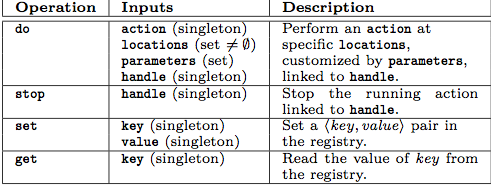
\includegraphics[width=\linewidth]{pictures/Voltron.png}
  \caption{Voltron APIs}
  \label{fig:voltron}
\end{figure}


The team-level approach represents a  middle-ground between the drone-level and swarm-level approaches, and it also solves many problems. Unlike the drone-level approach, there is no need to address the single drone and, unlike the swarm-level approach, there can be a "global state" and also time and space constraints can be defined; as already said, the team-level approach's main limitation is that there is no possibility to perform tasks which require explicit communication between drones, such as passing an object between them.
\\

\section{Data-flow programming}\label{dataflow}

Dataflow Programming is a useful programming paradigm that allows a developer to represent the execution model of his application through a directed graph. The flow of the data processed during the execution streams between all nodes. Each node is a functional block that accept data as input, manages it performing its tasks and then drive it forward to the next block. 
\\
The final dataflow application is nothing but a composition of these active blocks with at least one initial and one ending blocks, connected by directed arrows.
A block is connected to another when it has a dependency on the result of the manipulation of the data from that block. Values are propagated after they are processed from all the dependent blocks triggering their execution.
\\

This paradigm present some limits of expression.
The main one is that each implementation of this paradigm is specific for the context where it is used. This means that there are no general frameworks that can be used in more than one context. This is why we created our own dataflow editor, shown in Section \ref{plutoGraphicalEditor}.

\subsection{Business Process Modeling Notation}\label{BPMN}

Business Process Modeling Notation (BPMN) is an example of the power of the dataflow programming paradigm. Its primary goal is to help business users providing a readily understandable notation, filling the gap between the business process design and the final process implementation.
\\

BPMN defines a diagram that contains graphical models of the business process operations. A Business Process Model, is nothing but a graph where nodes represent graphical models representing the operations, and edges are the flow controls that define their order of performance. An example is shown in figure \ref{fig:bpmn}.
\\

 \begin{figure}[htbp]
   \centering
   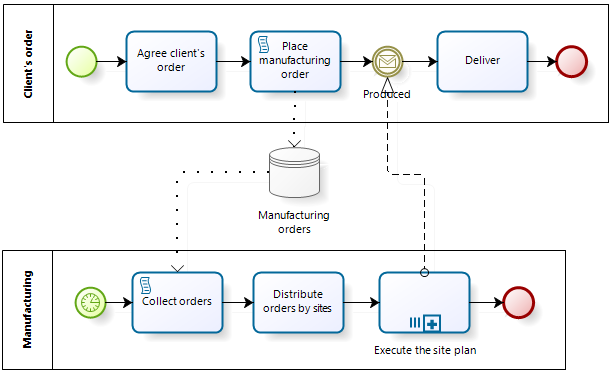
\includegraphics[width=\linewidth]{pictures/bpmn.png}
   \caption{Example of a BPMN diagram}
   \label{fig:bpmn}
 \end{figure}

There are different kinds of elements in a diagram:

\begin{itemize}
\item{\textit{Flow Objects}: they can be Events (circles), Activities (rounded rectangles) or a Gateway (diamonds)}
\item{\textit{Connecting Objects}: they can represent a Sequence Flow (solid line), a Message (dashed line) or an Association (dotted lines)}
\item{\textit{Swimlanes}: they can be a Pool representing the Actor of the process, or a Lane that is a sub-partition within a Pool}
\item{\textit{Artifacts}: they are useful to extend the basic notation adding new ways to describes context based information}
\end{itemize}

\subsection{Node-RED}\label{NodeRed}

Node-RED is an example of the dataflow paradigm applied to the \textit{Internet of Things} world.
It is a browser-based editor that let the developer wire together different nodes with directed edges.
Each node provides a different feature or a different management of the input data.
All features are web-based functionality, such as receiving an HTTP request or a \textit{Javascript} snippet.
In this context, a diagram represents the back-end of the web application and When the graph is completed, the user can deploy it with a single-click in the runtime environment.
The light-weight runtime is built on \textit{Node.js}, taking full advantage of its event-driven, non-blocking model. This makes it ideal to run at the edge of the network on low-cost hardware as well as in the cloud.
\\

In figure \ref{fig:nodeRed} we show an example web application:


 \begin{figure}[htbp]
   \centering
   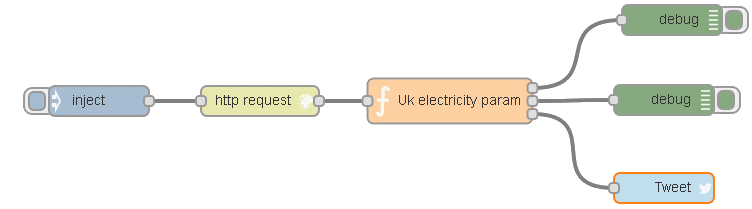
\includegraphics[width=\linewidth]{pictures/nodeRed.png}
   \caption{Example of a nodeRED application}
   \label{fig:nodeRed}
 \end{figure}

The yellow node makes a GET request to the UK electric company website.

The response data follow the edges and pass through the orange node, which lets the developer write its custom Javascript code inside it. 
In this case, the custom code takes the payload data in input and put them on the third output, formatting them in readable way. 
Through the first two outputs, the block sends only debug strings that go to the green nodes.
In the end the blue node will send a tweet containing the data received as input.
\\

In this Chapter we have described the actual state of the art in the field of drone programming and dataflow programming.
We needed to overcome the limits of the actual state of the art by performing some modifications to the existing solutions, which we show in Section \ref{teamlevelproblems}.




\chapter{Indoor applications using autonomous drones}
\label{cap3}

In this Chapter we show all the problems we had to face in the development of our programming framework. 
We first show a concrete application we wanted to develop, and then the problems deriving from its development.
No one of the existing drone programming approaches, shown in Chapter \ref{cap2}, is fully suitable for our problem.
We chose a Team-level programming approach, described in Section \ref{teamlevel}, but we had to perform some modifications on it, as we explain in Section \ref{teamlevelproblems}.
There are also some technological limitations, such as the lack of a stable indoor localization system and the short duration of nano-drones battery, which we explain in Section \ref{challenges}.

\section{Motivating scenario\label{motivating}}

In order to concretely show all the limitations and problems encountered in the development of our system, we start this Chapter describing a concrete scenario.
We want to develop an application to assist elders to take their medicines, for example in a hospital context.
A team of nano-drones could help the nurses to deliver the daily medicines to the patients at the right time of the day.
A representation of the behavior of the application, which we named Drugs Distribution(DD), is shown in figure \ref{fig:motivating}:


\begin{itemize}
\itemsep2pt
\item{
the nurses prepare the little boxes with each patient’s daily medicine
}
\item{
each drone, at the right time of the day, brings the box to its assigned patient
}
\item{
after carrying out their action, the drones return to the start location
}

\end{itemize}


\begin{figure}[H]
  \centering
  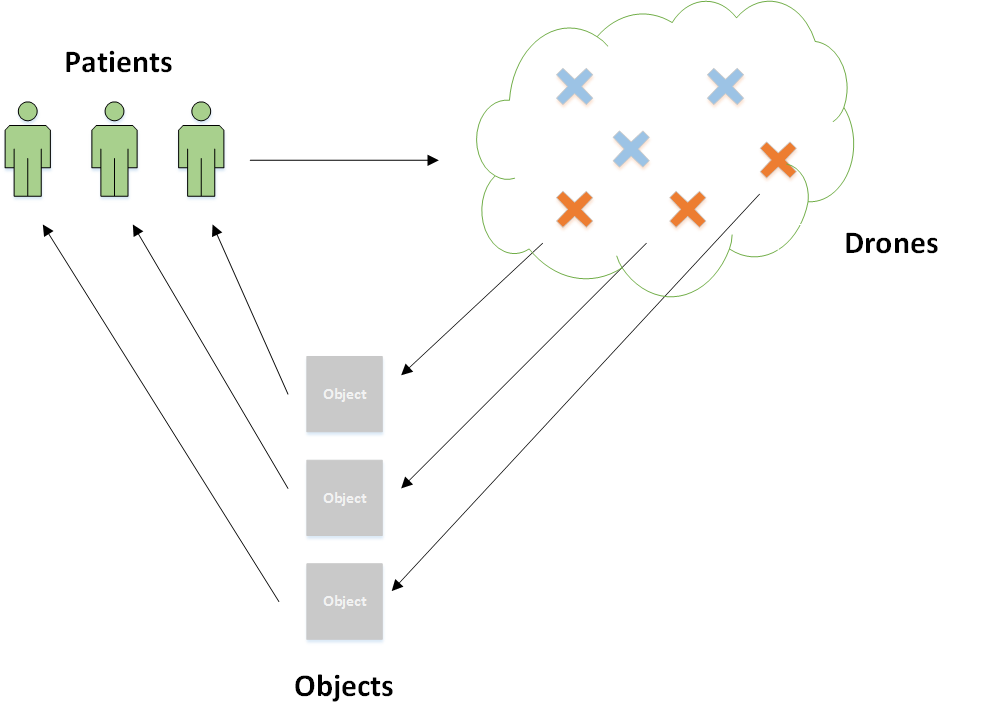
\includegraphics[width=\linewidth]{pictures/DD.png}
  \caption{The basic functioning of the Drugs distribution application}
  \label{fig:motivating}
\end{figure}

The development of this application made us to face some problems, both in the implementation of the system and in the technological lacks, which we describe in the next two Sections.


\section{Drone programming}\label{teamlevelproblems}

Since the approaches for programming drones we described in chapter \ref{cap2} are designed in a way that is impossible to describe an application through the concepts of Mission and Trip, we give our contribution to the state of the art creating a new framework based on these entities.
A \textit{Mission} is nothing but a list of sensing tasks to be performed sequentially in the environment.
Each one of these sensing tasks is a \textit{Trip}, that is a movement from a point A to a point B to perform an Action.

Neither the Drone-level nor the swarm-level approaches, described in Sections \ref{droneLevel} and \ref{swarmLevel} respectively, are suitable for our goal. 
The former because we do not want the user to deal with the coding of each drone separately with an external API.
The latter because we want to avoid the complexity to create a communication network protocol between drones and because it would be difficult to maintain the status of the missions and trips entities among the swarm. Moreover we also need to address  time and space constraints, which cannot be expressed with this approach.
\\

The most suitable approach for our framework is the Team-level model, described in Section \ref{teamlevel}, but we need to apply some modifications to it, in order to make it suitable for our work.
Using a Team level approach entails some problems:
the user can neither address individual drones nor express actions that involve direct interactions between drones, such as those required to pass an object between them.
This is the main limitation of the approach, but it does not directly affect the development of our DD application, described in Section \ref{motivating}.
So we have to modify the Team-level approach in order to make each drone deliver the box of medicine to its assigned patient, independently from the other drones. 
So we need the concept of \textit{Trip}.
A \textit{Trip} is nothing but a movement from a point A to a point B in the environment to perform an action.
In this way, we can tell each drone to go to the precise location of its assigned patient, making the Trip of each Drone independent from the others.
The concept of \textit{Trip} is a fundamental feature of our model, and it is fully described in Section \ref{programmingModel}.
\\

Another very important feature of our system is the transparent dispatching of drones:
the central brain takes care of assigning the drones to the sensing tasks to be performed, managing also the drones failures, without involving the programmer.
\\

Another problem of the Team-level approach is that, having a single brain which manages all the application logic and the dispatching of drones, the system get a single point of failure, so, if the central brain breaks then the whole system crashes.
This problem can be fixed or at least weakened by applying some dependable systems methods, improving reliability of the central brain, reducing its rate of failure etc.
\\

Even though team-level approach has his own limitations, other approaches we discussed in section \ref{cap2} are less suitable.
Indeed, the Drone-oriented approach, described in section \ref{droneLevel}, has the problem that the programmer has to manage individually the drone's movements and the interactions with other drones: he must code a list of instructions and commands that the drone will perform sequentially. This can only be achieved with the exploiting of specific API of each drones.
In the case of multiple drones,the programmer should deal with difficult programming tasks, like concurrency and parallelism, and it should also manage the drone batteries discharge and their crashes/failures.
Adding one or more drones to the system could complicate a lot the programming task. The programmer should also deal with timing constraints and he should balance the load between drones in a dynamic way.
Is clear that the drone-level approach is most suitable for applications involving only a few drones.
\\

On the other hand, the Swarm-level approach, described in section \ref{swarmLevel}, is more suitable for applications where there’s need of a lot of drones performing the same actions.
Indeed the programmer can give a set of basic rules that each drone should follow. It is important to underline that, in swarm-level approach, there is no possibility to have a shared state between drones; each one execute the actions specified by the programmer on his own local state. This means that this approach is very easy to scale up adding new drones, but it’s not suitable for applications that require the drones to explicitly coordinate.
\\

Regarding the dataflow programming, we need a new framework that allows the user to design the behavior of the central brain taking care of the missions execution, from the beginning to the end. 
This modeling tool helps the developer to add the features needed by the application simply drawing the proper nodes in the dataflow graph. 
The BPMN and Node-RED dataflow models, described in Sections \ref{BPMN} and \ref{NodeRed} respectively, are too general for our system, since they allow to model almost every kind of project.
They offer a great number of components, but we only need basic components for our editor, like rectangles and arrows.
So we decided to develop our own dataflow model, offering only the functionality and components needed for our programming framework.
This part of the project is fully described in Section \ref{plutoGraphicalEditor}.

\section {Implementation challenges}\label{challenges}

The DD application, shown in section \ref{motivating}, makes drone bring medicines to the elders in an hospital, so in an indoor context.
One big problem is that there is not a stable localization method for the indoor environment.
Besides of localization problem, indoor context also leads to the limits of the size of the drone.
As a result, programmers constantly confront with a limited battery resource and a small weigh the drone can carry out. These problems, as well as their possible solutions, are described in the following Section.

\subsection{Indoor localization}

The main issue that all developers are facing, working on an indoor application for drones, is that they are not able to use the Global Positioning System (GPS); it cannot be used because of walls,roofs or ceilings.
For this reason Indoor Positioning System(IPS) is widely applied for indoor localization. In this section we will give an overview of existing IPS methods.  
\\

An indoor positioning system is a solution to locate objects or people inside a building using radio waves, magnetic fields, acoustic signals, or other information collected from the sensors of mobile devices.
The IPS methods rely on alternative technologies, such as \textit{magnetic positioning} and \textit{dead reckoning}, to actively locate mobile devices and provide ambient location for devices to get sensed.

Today many IPS methods have been developed and they can be divided in two main categories: \textit{Non-radio technologies} and \textit{Wireless technologies}.
\\

Non-radio technologies have been developed for localization without using the existing wireless infrastructures, and they can provide very high accuracy.
Nevertheless, they also require expensive installations and costly equipment.
\\

For example, \textit{Magnetic positioning}\cite{magnetic} is based on the iron inside buildings that create local variations in the Earth’s magnetic field.
Modern smartphones can use their magnetometers to sense these variations in order to map indoor locations.
\\

With \textit{Inertial measurements}\cite{IMU} pedestrians can carry an inertial measurement unit(IMU) by measuring steps indirectly or in a foot mounted approach, referring to maps or additional sensors to constrain the sensor drift encountered with inertial navigation.
\\

Existing wireless infrastructures can be used for indoor localization; almost every wireless technology is suitable, although they are not as precise as non-radio technologies.
Localization accuracy can be improved at the expense of new wireless infrastructure equipment and installation.
WiFi signal strength measurements are extremely noisy, so there is need to find a way to make more accurate systems by using statistics to filter out the inaccurate input data. WiFi Positioning Systems are sometimes used outdoors as a supplement to GPS on mobile devices, where only few reflection phenomena could happen.
\\

\textit{WPS}\cite{WPS} is based on measuring the intensity of the received signal(RSS) together with the technique of \textit{fingerprinting}.
In computer science, a fingerprinting algorithm is a procedure that maps an arbitrarily large data item to a much shorter bit string, its fingerprint, that uniquely identifies the original data for all practical purposes just as human fingerprints uniquely identify people for practical purposes.
The accuracy of WPS improves with the increase of the number of positions entered in the database.
WPS is subjected to fluctuations in the signal, that can increase errors and inaccuracies in the path of the user.
\\

\textit{Bluetooth}\cite{bluetooth} cannot provide a precise location, since it's based on the concept of \textit{proximity}, indeed it is considered an \textit{indoor proximity solution}.
However, by linking micro-mapping and indoor mapping to Bluetooth and through the usage of \textit{iBeacons}, real existing solutions have been developed for providing large scale indoor mapping.
\\

It is important to underline that we made the choice to decouple the system working logic from the \textit{Navigation System}. The navigation system is the module of our central brain that makes use of indoor localization API, providing to the central brain a way to control the drones with accurate coordinates. In this way all previously described technologies are suitable with our system, on condition that the developer provides the proper API.
\\

\subsection{Drones and Objects size limitation}

Indoor contexts imply small areas which are usually full of people and obstacles hence, drones have to be small, in order to avoid crashes with both human and environmental obstacles.

Size limitations result in many problems; the first is battery duration, which can reach a maximum of 8 minutes, having a recharge time of about 20/30 minutes.
It limits the programmer in developing applications which require the drones to perform their actions in this limited amount of time.

Another problem arising from size limitations is that the smaller the drone is the less stable he is.
Almost every kind of micro-drone has serious stability issues, and a lot of research efforts goes in this direction. This problem is lowered by the developing of programming libraries that could improve stability of the drones at real-time, adjusting a set of parameters while the drone is flying.

Micro-drones are obviously more fragile than the big ones, so a crash with humans or obstacles can definitely destroy the drone or make it seriously damaged. This is the price to be paid for having little drones that can operate in small indoor contexts.

Finally, the use of small drones means that only small objects can be taken, so the applications developed with Pluto framework must take this into account.
For example, a pair of keys can be brought to a person, not a book nor a pair of shoes.
\chapter{Programming with Pluto}
\label{cap4}

In this chapter we present our solution to the issues introduced by the indoor context, its system architecture and, in the last section, how we achieved this result. We already said our goal is to complete user-defined missions, using nano-drones in an indoor context. We chose the Team Level approach, which we described in section ~\ref{teamlevel} to manage the missions assignment because, as we have shown in Section~\ref{teamlevelproblems}, the Team-Level approach is the most suitable approach for the kind of applications that can be developed with our framework.
The most important advantage of this approach is the reduced complexity given to the final user, while expressing the sensing tasks: there is no need to describe how the drones should execute them; these details are chosen by the Ground Control Station whose duty is to assign the right drone to the right task and check that each drone take its mission to the end with a successful status.


\section{System's architecture}
Pluto programming framework consists in two main components:
\begin{itemize}
\item Pluto Graphical Editor.
\item Pluto Main Application.
\end{itemize}
The former is used by the first actor of the Pluto life-cycle: a developer. The latter is used by a final user whose duty is to insert the sensing task and start their execution.
As you can see in figure \ref{fig:lifeCycle}, Pluto Graphical Editor lets the developer to creates a scenario based on the Team Level approach as we show in Section ~\ref{plutoGraphicalEditor}. After that, the Pluto Main Application is generated based on the diagram created in the previous step, so that the final user needs only to insert the sensing task and wait for their accomplishment.

\begin{figure}[htb]
  \centering
  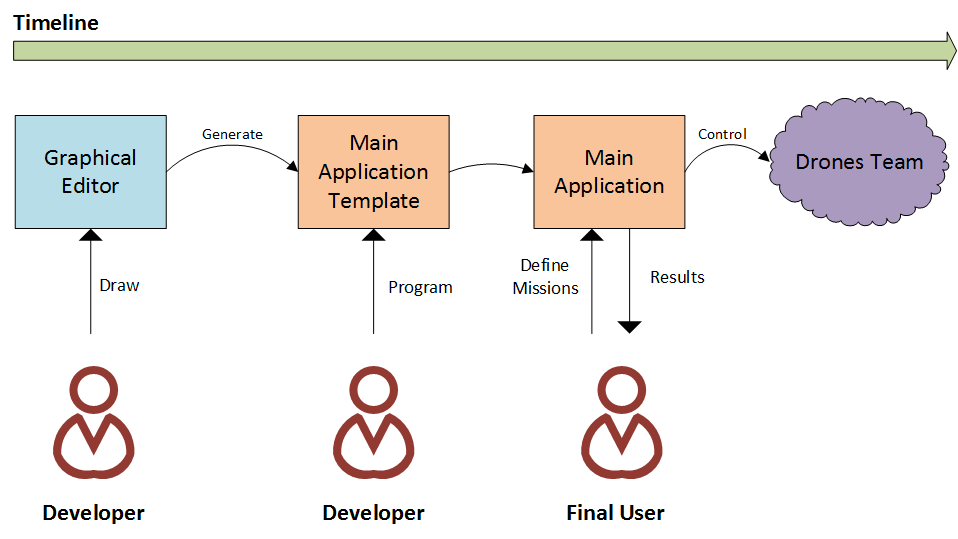
\includegraphics[width=\linewidth]{pictures/lifeCycle.png}
  \caption{A complete life cycle of the application}
  \label{fig:lifeCycle}
\end{figure}

\subsection{Pluto Graphical Editor}
\label{plutoGraphicalEditor}

We created a Graphical Editor in order to give freedom to the developer while designing the final app. The provided tools can be used to link together different kind of blocks, each one with a predefined and implemented logic.
When the Editor starts, it shows three main sections: the Palette that contains all the tools available to create a fully functional diagram; the Editor space, where the user can move, link, manage all the created entities; last but not least is the outline with a tree-view of the blocks created by the developer in the editor space.

\begin{figure}[htb]
  \centering
  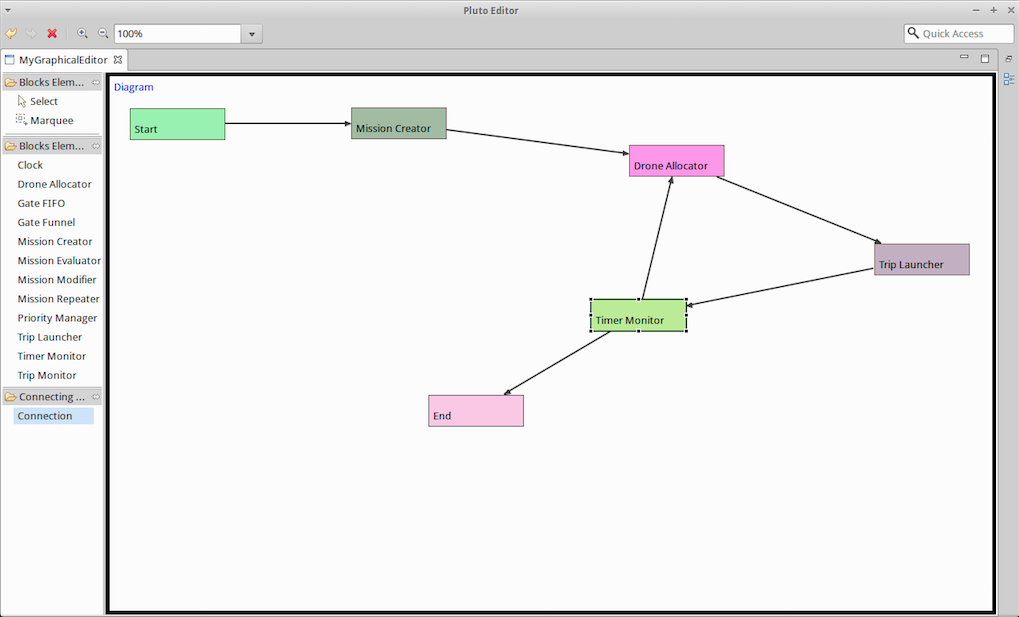
\includegraphics[width=\linewidth]{pictures/EditorScreen.png}
  \caption{Pluto Graphical Editor interface}
  \label{fig:GraphicalEditor}
\end{figure}

The developer can choose among several types of pre-created blocks, each one containing a certain logic, explained in (section~\ref{entities}). Creating a block in the editor space can be done simply with a drag and drop gesture or clicking on the desired entity and then clicking on the chosen location in the editor. Then the user can connect blocks each other using the Connection tool in the Palette section.
Apart from the standard functionality, such as Undo, Save, and Load, the Context Menu provides a command to generate a source-code of the Main Application based on the designed diagram. Toolbar provides Undo/Redo, Delete, and Magnify commands.
To understand better Pluto Graphical Editor, it's worth to spend a word on the meaning of creating a diagram: each block in the Diagram is black box which is intended to manage a Mission entity. It takes a Mission as an input, works with it and sends it out as an output. The connections among blocks represents the path that the Mission entity will follow after going out from a block. Each block could have multiple outgoing and incoming connections.
In the end, on the editor, the developer will have a set of blocks linked together with a set of connections. This drawing can be interpreted as the behavior of the Main Application in managing the missions. For example we designed a sketch of a possible diagram, as shown in figure ~\ref{fig:GraphicalEditor}. This design is very simple and could be a first skeleton for a more complex application, by simply adding new blocks.
Besides of simplicity, our editor is very flexible as well, since it provides a Mission Modifier block whose implementation logic can be written directly in the Editor right-clicking on the block and choosing the option "Write Custom Code". This will be explained better in section~\ref{entities}

\subsection{Pluto Main Application}
\label{plutoMainApp}

The Pluto Main Application is the final application that act as a Ground Control Station, managing all the drones and the missions. In this section we explain how it works.
Everything starts in the Mission Page where the user can define the tasks that will be carried out by the drones. After clicking to the "Add Mission" button the user is asked to set a name for the mission.

\begin{figure}[htb]
  \centering
  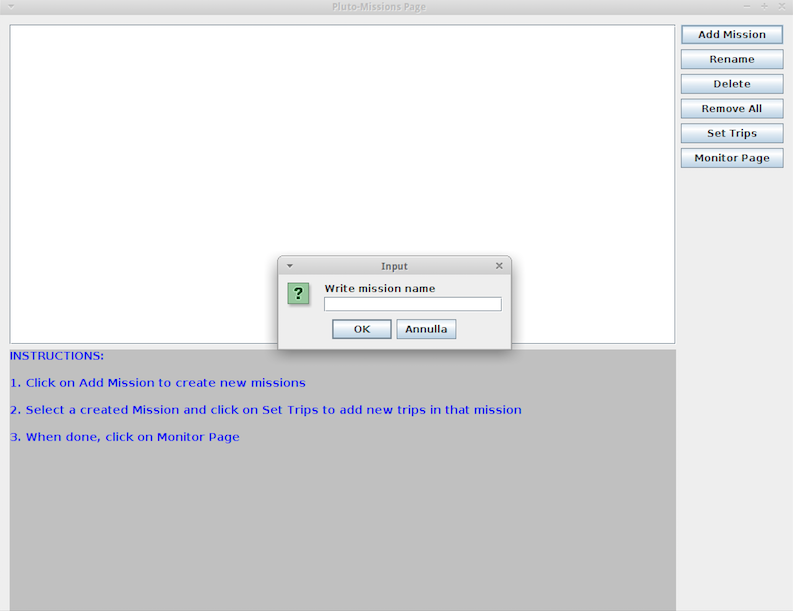
\includegraphics[width=\linewidth]{pictures/MissionPage.png}
  \caption{Mission Page interface}
  \label{fig:MissionPage}
\end{figure}

Then, the user is asked to decide if the mission must be repeated. If he click "Yes", that mission will continue to execute cyclically until the user decide to stop it, through the Stop button of the Monitor Page.

\begin{figure}[htb]
  \centering
  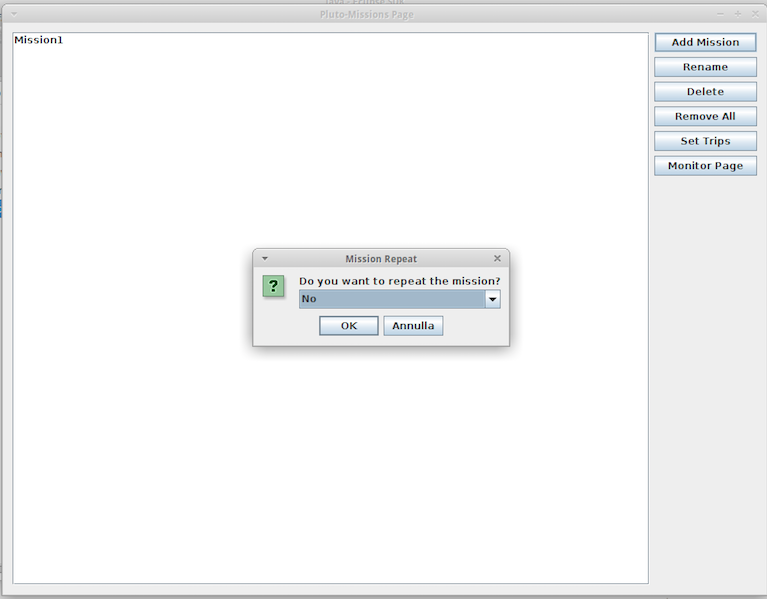
\includegraphics[width=\linewidth]{pictures/missionRepeat.png}
  \caption{Mission Repeatable pop up}
  \label{fig:missionRepeat}
\end{figure}

After that a Mission entity is created, but by now it doesn't contain any information about what has to be done. To add this information the user has to double-click on the mission in the main list or click on the "Set Trips" button. A new window will appear, as shown in figure  ~\ref{fig:TripsPage}, and the user can add Trips entity to the related Mission. A Trip is nothing but a movement from point A to point B inside our indoor context. Trips are the basic entities that constitute a single Mission. The single Trip contains information about the Action to execute once point B is reached. Furthermore the Trip has a reference of the drone assigned to it, but we will talk about this in section ~\ref{entities}.

\begin{figure}[htb]
  \centering
  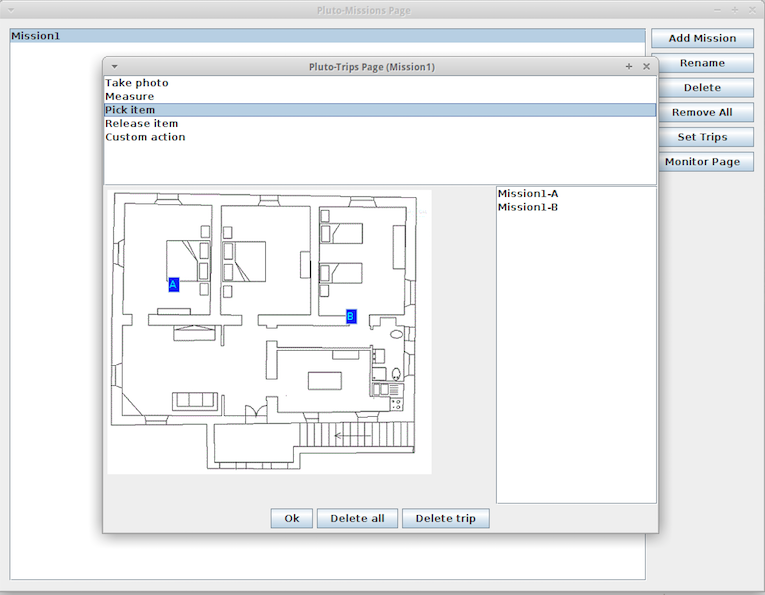
\includegraphics[width=\linewidth]{pictures/TripsPage.png}
  \caption{Trips Page interface}
  \label{fig:TripsPage}
\end{figure}

So after all the Trips are added to a single Mission the user can create more Mission or pass to the Monitor Page with the corresponding button.
The Monitor Page, shown in figure ~\ref{fig:MonitorPage}, is the window where the user can obtain information about the running missions, at run-time. On the top, there is a table where each row is assigned to a Mission, each column will display the information about the current Trip that is executing and the Drone that has been assigned to that Trip.
Below the table there is a console where log messages are printed during the execution of each missions. In this way the user can obtain run-time information about the status of the entire system. 
Of course the Start button will start the execution of the created missions, while the Stop button will prompt the user to a behaviour choice: "RTL" or "Land". The first will make all drones to return to the home location instantly, while the second option will make all drones to land in their current locations. After the Stop command, the missions status will be preserved and could be continued in the future.

\begin{figure}[htb]
  \centering
  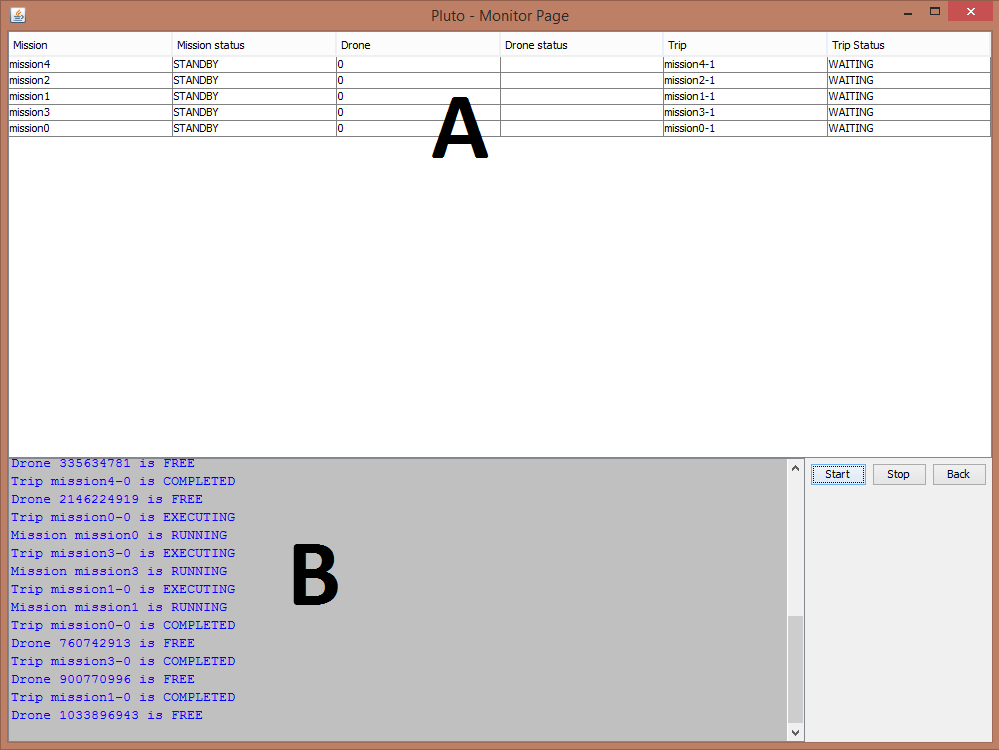
\includegraphics[width=\linewidth]{pictures/MonitorPage.png}
  \caption{Monitor Page interface}
  \label{fig:MonitorPage}
\end{figure}

\newpage

\section{Dataflow model}\label{dataFlow}

In this section we present the Dataflow model in a complete and sound way.
First, we describe a general view of the model in Section ~\ref{descriprionOfModel}. Then, in Section ~\ref{modelRepresentation} we focus on the details of the each component of the model.


\subsection{Description of the model}
\label{descriprionOfModel}

Each diagram created with the Pluto Graphical Editor is made of many functional blocks, each one is implemented with a particular logic; the user can select the blocks needed for his particular application and connect them through simple links, as explained in section~\ref{plutoGraphicalEditor}.
In the figure~\ref{fig:BlocksDiagram}, an example application is showed, which contains some of the implemented blocks.
Again, the user is not forced to insert all the blocks, he can choose only the blocks needed for his particular application.
If you compare this figure with figure~\ref{fig:GraphicalEditor}, you can see that this one is based on the the same drawing but with additional features provided by new blocks.
\\

\begin{figure}[htb]
  \centering
  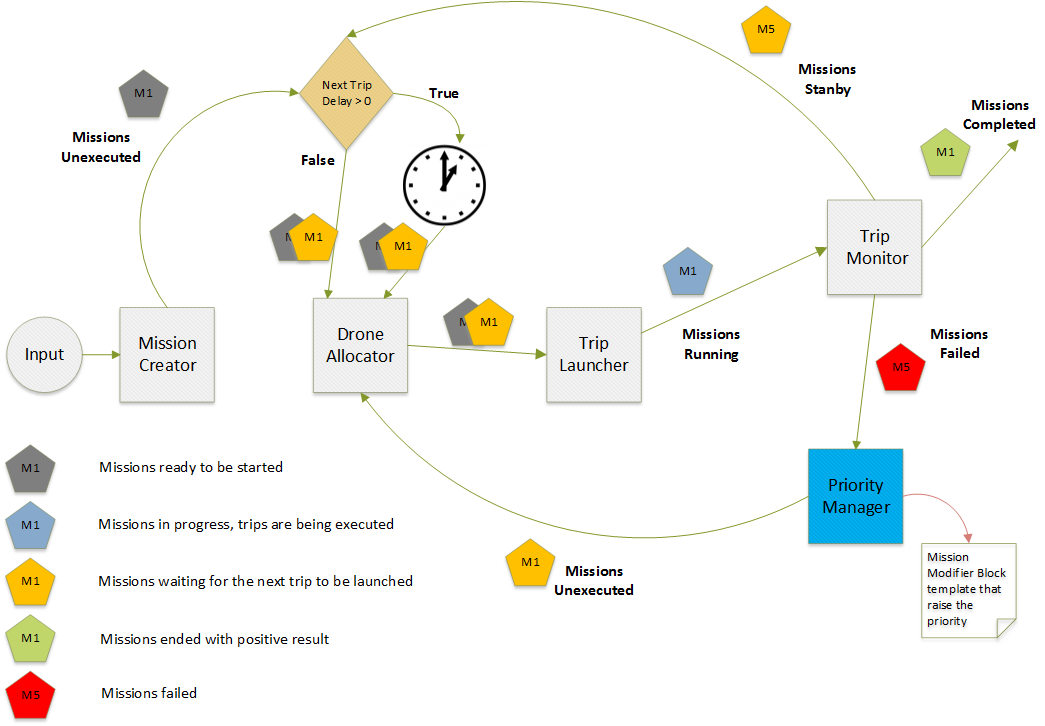
\includegraphics[width=\linewidth]{pictures/BlocksDiagram.png}
  \caption{An example Pluto application}
  \label{fig:BlocksDiagram}
\end{figure}


\newpage
\subsection{Model representation}
\label{modelRepresentation}
In this section we show the fundamental entities of our model, in order to better understand the functioning of the blocks. Then, all the blocks of figure ~\ref{fig:BlocksDiagram} are described in details, explaining what tasks they perform and showing a pseudo-code representation for each of them.

\subsubsection {Entities}
\label{entities}

Basically, through the interface presented in section~\ref{plutoMainApp}, the user specifies a list of Missions that the system must perform; each Mission contains a list of Trips; a Trip is a path between a start location and a target location; the Trip is performed by a Drone which carries out an Action, for example it can bring an Item to a person, or take a photo or measure temperature at a particular location.

So we identified the following entities:

\begin{itemize}
\itemsep2pt
\item{
Mission
}
\item{
Trip
}
\item{
Drone
}
\item{
Action
}
\item{
Item
}
\end{itemize}

As shown in figure~\ref{fig:EntityRelationship}, the Mission entity, in addition to the set of Trips, has another important attribute that is the Status: it describes how the Mission is being executing.
\\
The Trip entity has a Status attribute too and furthermore it contains the Drone and the Action entities. Then of course the coordinates of the source and the target locations.
\\
The Drones are described by an unique ID and by a shape category which tell the system what kind of items can be hold by the drone.
\\
Regarding the Action entity, a very important feature is the \textit{Custom Action}: it allows the programmer to implement a new action that the drones can perform.
It obviously depend on the particular application, but for example a programmer can add the Pollinate action needed for the Alfalfa application\cite{alfalfa}, which will be described in section \ref{alfalfa}.
\\
The code implementation of these classes can be found in section~\ref{oomodel}.

\newpage

\begin{figure}[htb]
  \centering
  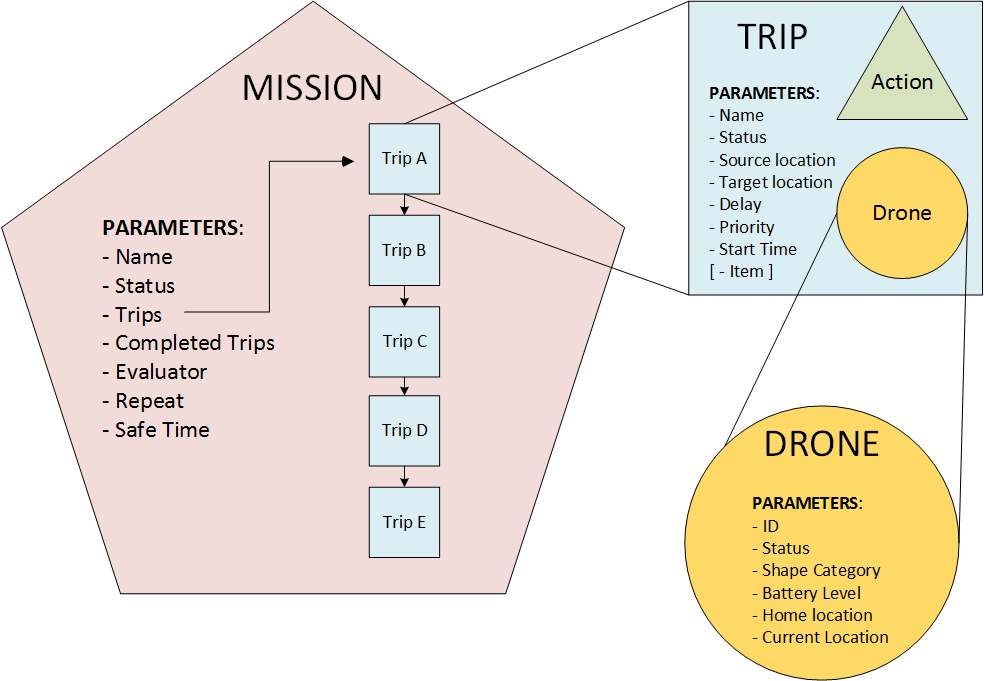
\includegraphics[width=\linewidth]
  {pictures/EntityRelationship.png}
  \caption{Relationship among model entities}
  \label{fig:EntityRelationship}
\end{figure}


\subsubsection {Description of the blocks}\label{blocks}

Here we provide a detailed description of each functional block available in the Pluto Graphical Editor:
\\

\underline{Mission Creator block}
\\

input: a list of Trips

output: a Mission object
\\

The Mission Creator block receives as input the trips that the user wants to be performed by the drones, then it creates a Mission including all these trips and returns that Mission object.
This block is the starting point of each Pluto-developed application.
\\



\underline{Clock block}
\\

input: a Mission object

output: a Mission object
\\

The Clock block checks the delay attribute of each Trip of a Mission: if it's not equal to zero, it makes the Trip wait for the amount of time set by the user in the Mission creation step, and finally returns the Mission Object.
If the programmer puts the Clock block in the graph of the application, the Pluto Main application shown in section \ref{plutoMainApp} will show an extra widow.
On the Trips Page,after the final user drags and drops on the map the action to perform and the Priority panel is shown, the user will be asked to set a delay for the Trip.
This block has to be put between the Mission Creator and the Drone Allocator blocks.
\\

\underline{Drone Allocator block}
\\

input: a Mission object

output: a Mission object
\\

The DroneAllocator block chooses the appropriate Drone to be assigned to each Trip, basing on the availability of the drones and their capability to perform the desired action.
The output of the DroneAllocator is always sent to the TripLauncher, while its input can arrive from a variety of blocks, depending on the features of the considered application.
\\

\underline{Trip Launcher block}
\\

input: a Mission object

output: a Mission object
\\
The TripLauncher block takes the next Trip to be performed from the Mission object, and launches it.
The assigned drone will fly to the target location and execute the defined Action.
This block receives the input Mission from the DroneAllocator block, ans sends its output to the TripMonitor.
If the application contains the TimerMonitor block, the TripLauncher's output will be also sent to it.
\\

\underline{Trip Monitor block}
\\

input: a Mission object

output: a Mission object
\\

The TripMonitor block checks the status of the Trip that is running in that moment.
It changes the status of the Trip and of the Mission in the appropriate way, depending on whether the Trip is failed or complete.
This block receives the input Mission from the TripLauncher, and its output can be sent to the GateFIFO, the MissionEvaluator or the DroneAllocator blocks, depending on the features of the particular application.
\\



\underline{Mission Repeater block}
\\

input: a Mission object

output: a Mission object
\\

The MissionRepeater block verifies if the \textit{repeat} attribute of the input Mission is set to true.
If so, it set the Mission status to STANDBY and the status of all the Trips of that mission to WAITING and inserts again them in the List of Trips to be executed.
This block is put between the MissionEvaluator and the DroneAllocator.
\\

\underline{Gate FIFO block}
\\

input: a Mission object

output: a Mission object
\\

The GateFIFO block is used when two or more blocks works in parallel, and only one instance of the executing Mission must propagate.
Among the multiple input connections of the GateFIFO block, it propagates only the one that completed its task for first.
That's why the FIFO acronym is used, since the first Mission instance that arrive is the only one that propagates in the graph.
This block receives the input Mission from one of the blocks connected to it and can send its output to the MissionEvaluator, MissionRepeater or DroneAllocator blocks, depending on the particular application.
\\

\underline{Mission Evaluator block}
\\

input: a Mission object

output: a Mission object
\\

The MissionEvaluator block can read and write data carried by the drones, and basing on them can perform various actions specific for the application developed.
It receives the input Mission from the GateFIFO or TripMonitor blocks and can send the output to the DroneAllocator or MissionRepeater blocks, depending on the particular application.
\\

\underline{Mission Modifier block}\label{mm}
\\

input: a Mission object

output: a Mission object
\\

The MissionModifier block allows the programmer to create new custom blocks.
As shown in figure~\ref{fig:missionmodifier}, in the editor, he can inserts his custom code in this block using the appropriate option in the context menu.
This block can be put in every point of the Pluto Editor graph, depending on the particular feature it implements.
\\

\begin{figure}[H]
\centering
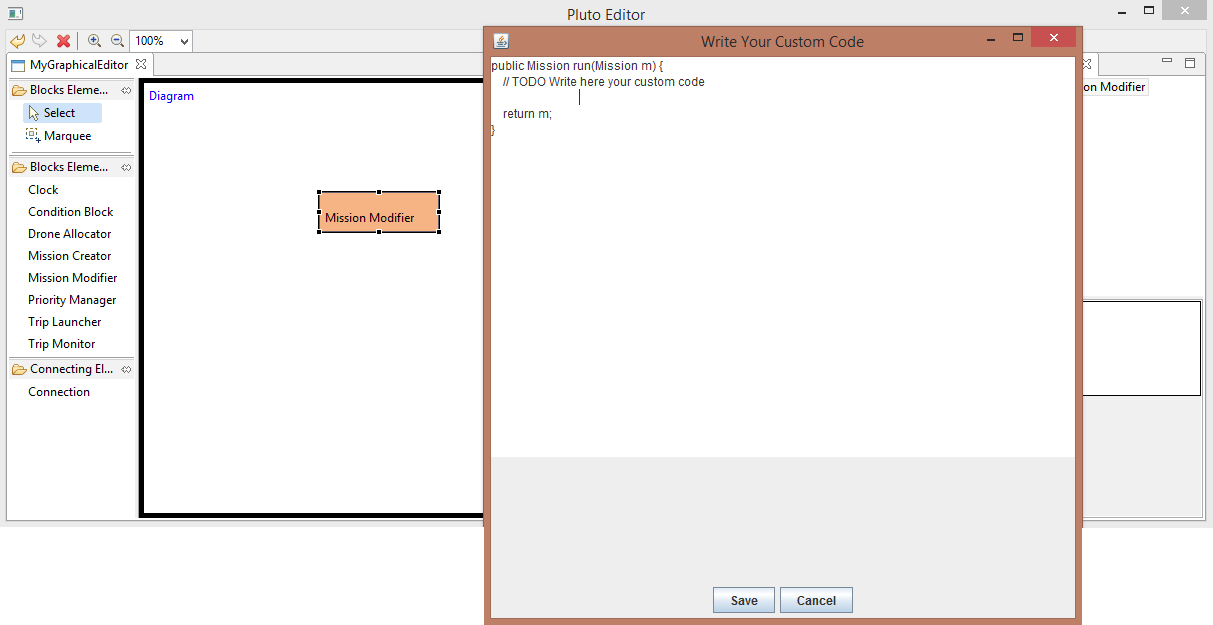
\includegraphics[width=\linewidth]
{pictures/MissionModifier.png}
  \caption{The MissionModifier block}
  \label{fig:missionmodifier}
\end{figure}

\underline{PriorityManager block}
\\

input: a Mission object

output: a Mission object
\\

The Priority Manager block raise the priority of the first Trip of the Mission passed in input.
This block can be considered as a particular case of Missio nModifier. 
This block can receive the input from the Gate Fifo or Trip Monitor blocks, and sends the output to the Drone Allocator.
\\

\underline{Timer Monitor block}
\\

input: a Mission object

output: a Mission object
\\

The TimerMonitor block takes the input mission and waits for the completion of the current running Trip. If the Trip doesn't end before the fail-safe time, it will set the status of the Trip and of the Mission both to FAILED, then it will put the mission as output.
This block can be considered as a particular case of MissionModifier.
It's always put between the TripLauncher and the GateFIFO blocks.
\\

\underline{Gate Funnel block}
\\

input: a Mission object

output: a Mission object
\\

Similar use of the GateFIFO, but this gate will wait for all the Mission instances that are being managed before this block. So if before this gate, there are 4 blocks in parallel that are managing their Mission instance, the propagation of the Mission after this gate will be activated only when all the 4 instances will arrive.
\\

\underline{Start block}
\\
State the beginning of the diagram
\\

\underline{End block}
\\
State the end of the diagram, where the completed missions will go into.
\\

\section{Aiming to the final model}

In this section we describe our previously developed solutions, which we refined many times in order to obtain the final working version of the Pluto programming framework; this is done by using a top-down approach, starting from the final implementation to the very first one.

\subsection{Solution without Trip entity}

In the version precedent to the final solution, presented in section~\ref{dataFlow}, we did not have a concept of Trip, and Mission was the main concept the whole model was based on. The following diagrams shows this in the particular case of the Timer feature, which contains also a "Switch source-target" block. Later, this block was included in the logic of the Trip.

\begin{figure}[htb]
  \centering
  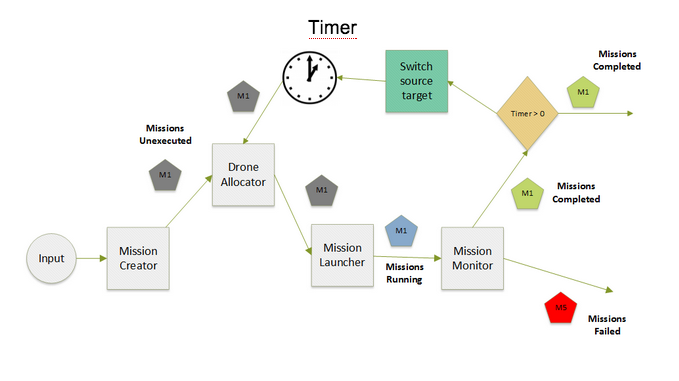
\includegraphics[width=\linewidth]{pictures/NoTrip.png}
  \caption{Solution without the Trip concept}
  \label{fig:noTrip}
\end{figure}

After analysing the model, we realized that we needed the concept of Trip, because the final user must have control on the single Trip of a drone, in order to decide which action the drone must perform, and to have an opportunity to control the Trip such as delay, stop, or delete, without deleting or stop the whole Mission. With this precedent solution it is not possible, because having only the entire  Mission to manage, the user can no control the single Trip, and if he/she wants to delete only a part of the Mission he cannot do so, and he/she is forced to delete and build again the whole Mission.

\subsection{Solution without the DroneAllocator}


This solution instead of the DroneAllocator block, used the "Drone Updater" one. This block managed the assignment of the Drone to a Mission, only in special conditions. This means that, generally, there were no need of this block unless the developer put some special block such as the old TimerMonitor or the old DelayMonitor.
In this solution, the MissionCreator managed the assignment of a Drone to the Mission. This is the reason why we didn't need the DroneUpdater in normal conditions.
As said, there were also the "Delay Monitor" and "Timer Monitor" blocks, instead of the Clock block.
These blocks managed the delayed missions(fig.~\ref{fig:delayMonitor}) and the missions with an associated timer(fig.~\ref{fig:noClock}), respectively.
There wasn't the MissionModifier block, but only the "Priority Manager" one, so the programmer couldn't insert blocks(fig.~\ref{fig:noMM}) with custom code.

\begin{figure}[htb]
  \centering
  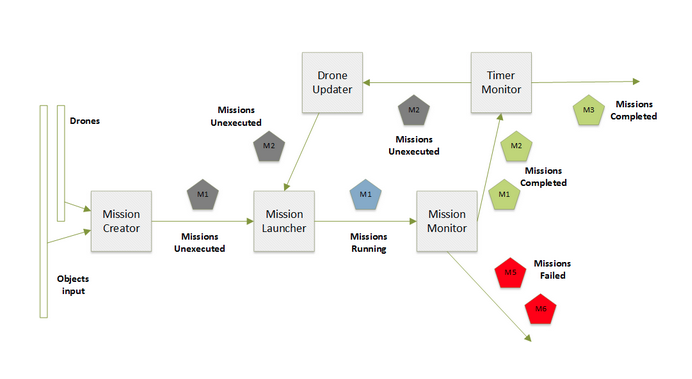
\includegraphics[width=\linewidth]{pictures/NoClock.png}
  \caption{Solution with the TimerMonitor}
  \label{fig:noClock}
\end{figure}


\begin{figure}[H]
  \centering
  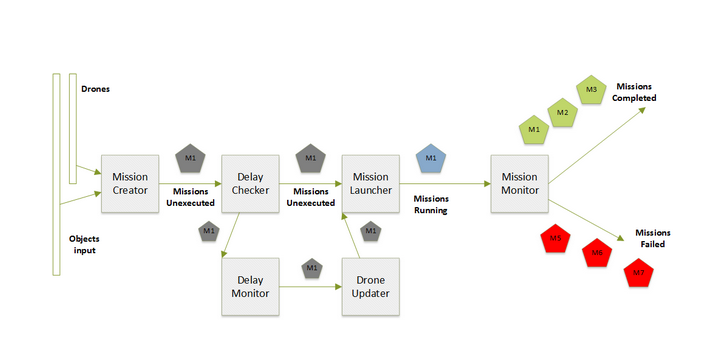
\includegraphics[width=\linewidth]{pictures/DelayMonitor.png}
  \caption{Solution with the DelayMonitor}
  \label{fig:delayMonitor}
\end{figure}

\begin{figure}[htb]
  \centering
  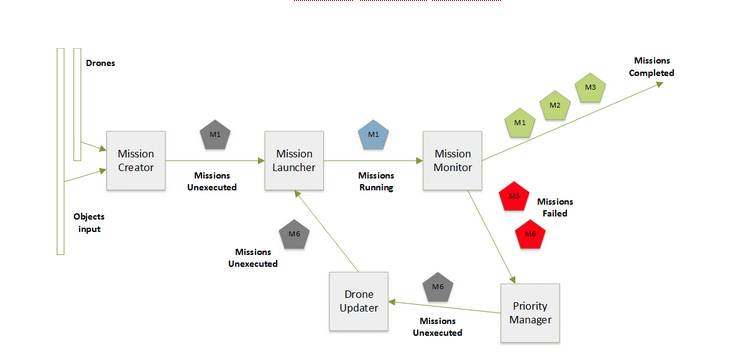
\includegraphics[width=\linewidth]{pictures/NoMM.png}
  \caption{Solution without the MissionModifier block}
  \label{fig:noMM}
\end{figure}

Actually we decided to put the DroneAllocator block because weneed to separate the creation of a Mission Object from the assignment of a Drone to it; in this way we could also remove the DroneUpdater block, because now we have an apposite block which manage only the assignment of Drones, so there is no more need to distinguish between the normal assignment and the special assignment(in the case of delayed trip).
Also the DelayMonitor and TimerMonitor blocks were useless, because there is no need to distinguish between a delay and a timer, so a single Clock block can manage these cases both.
In this solution only the PriorityManager block existed, but we decided to create a MissionModifier block in which the user can put his own code he needs for a particular application, so the PriorityManger block can be seen as a particular case of the MissionModifier one.
\chapter{Implementation}
\label{cap5}

In this chapter we show how we implemented the Pluto Framework, describing the main elements of the project separately, in order to better understand their behaviors.
In figure \ref{fig:finalArchitecture}, we show the final architecture scheme that includes all the parts described in the following sections.
\\

\begin{figure}[h!]
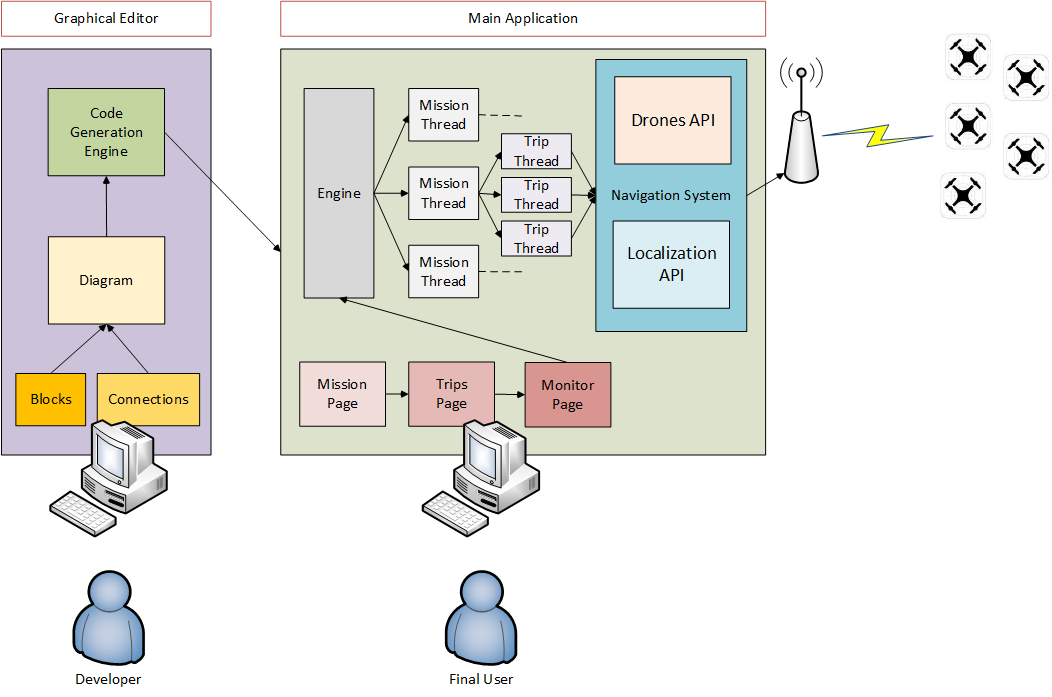
\includegraphics[width=\linewidth]
{pictures/Final_Architecture.png}
\caption{Pluto architecture representation}
\label{fig:finalArchitecture}
\end{figure}

\section{Object-oriented approach}\label{oomodel}

We used the Java programming language to implement both the Graphical Editor and the Main Application.
We made this choice because we are very familiar with Java, since almost every academic project we implemented in these years made use of this Object-Oriented programming language.
The Object-Oriented approach perfectly suits the Pluto model, since we have different independent entities such as Drones,Missions and Trips that interact together in the execution of tasks.
\\

We decided to adopt a Model View Controller(MVC) approach.
The central component of MVC, the model, captures the behavior of the application in terms of its problem domain, and it is independent from the user interface.
The model directly manages the data, logic and rules of the application.
A view can be any output representation of information, such as a chart or a diagram; multiple views of the same information are possible.
The third part, the controller, accepts input and converts it to commands for the model or view.
\\

\begin{figure}[h!]
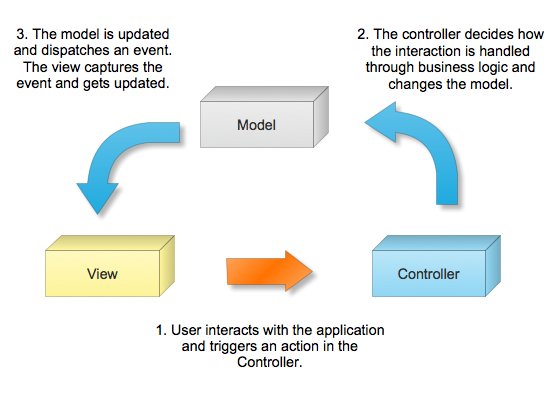
\includegraphics[width=\linewidth,height=9cm]
{pictures/MVC.png}
\caption{MVC design applied to the Main Application}
\label{fig:mvc}
\end{figure}

As shown in figure \ref{fig:mvc}, the model part contains all the Java classes of the entities shown in Section \ref{programmingModel}.
There is a class for the Mission, one for the Trip etc.
The controller part contains the Java classes of all the blocks of the Graphical Editor shown in Section \ref{functionalBlocks}.
The controller part also deals with the threads management needed for the execution of both the missions and trips. The thread structure is shown in Section \ref{runtimeMng}.
The view part contains the Java classes of the three pages of the Main Application shown in Section \ref{plutoMainApp}.
\\

\section{Graphical editor}\label{editor}

In order to create the Graphical Editor, described in Section \ref{plutoGraphicalEditor}, we decided to use the GEF (Graphical Editing Framework) project. This framework is a Java technology and it is part of the Eclipse framework developed by IBM.
\\

It gives developers a full solution for the graphical modeling of a Java object model, and it can be used in conjunction with other technologies such as EMF (Eclipse Modeling Framework) or GMF (Graphical Modeling Framework), to enable the creation of a complete graphical modeling suite. 
This means that the Pluto Graphical Editor has been developed as an Eclipse Plugin, so the developer has to install the Eclipse IDE in order to exploit the editor.
\\

First of all, we created the Java classes of all the blocks.
Each class contains the code implementation of the corresponding block, since each block perform a specific functionality.
We defined each block as a rectangle figure, then we added the connection entity in order to enable links between them.
All these entities are children of a main container class that represents the diagram itself that is simply a container for the graph.
Figure \ref{fig:editorExplanation} shows these components: A is the diagram entity, the container of the graph; B is the connection entity, through which the user connects the blocks; C is the block entity. 
\\

\newpage

\begin{figure}[h!]
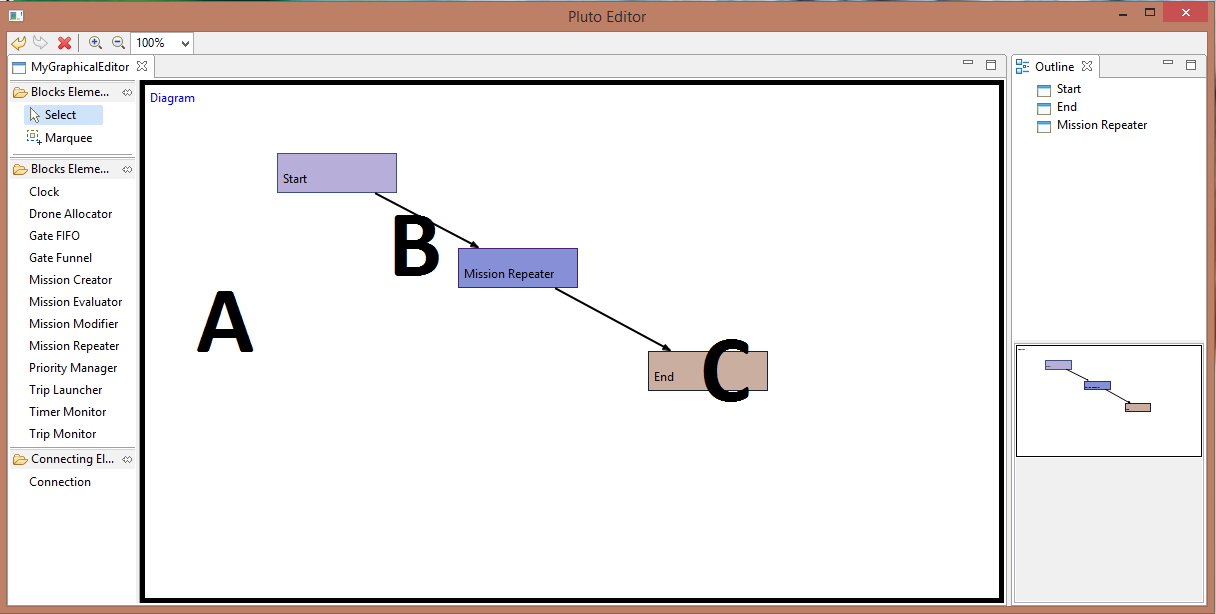
\includegraphics[width=\linewidth]
{pictures/editorExplanation.png}
\caption{Graphical entities in the editor}
\label{fig:editorExplanation}
\end{figure}

When the user creates a new  block in the editor area, a relative block entity is automatically created and added to the diagram container class. The same operation stands for the connections creation.

After the user draws the desired graph he can choose to generate the final code of the Main Application, through the apposite voice in the context menu.
See Section \ref{codeGeneration} for further details.
\\

\section{Code generation}\label{codeGeneration}

Once the programmer has created the graph of the application through the Pluto Graphical Editor, he can generate the code in order to make the Pluto Main Application behavior coherent with the graph.

This can be done by right clicking on the graph and choosing the "Generate code" command.

The main issue in the generation process was to understand how to generate the code from a general diagram. 
Potentially, a developer could draw a very complex graph with lot of blocks and connections between them.
At first, we focused on graph exploration methods, but we immediately noticed that they were too complex.
\\

So, we decided to adopt a \textit{Publish-Subscribe} design, making use of the \textit{Observer} pattern. This mechanism let us describe the execution flow of very complex diagrams, besides the more simple ones.
\\
 
The \textit{Observer} pattern consists in the declaration of some elements as \textit{observers} and of other entities as \textit{observable}. 
When an observable object change its status, it sends a notification to all its observer entities. 
These observers react according to the change of the observable object.
\\

In Figure \ref{fig:observerPattern} there is a sequence diagram that describes how the observer pattern works with a simple diagram with four blocks (A, B, C and D).
\\
The "Observe" message in the sequence is the declaration of a block that wants to observe another block. The "Notify" message represents the notification that a block sends to its observers when it changes its status, or in this case when the block ends the management of the Mission object.
\\

 \begin{figure}[h!]
 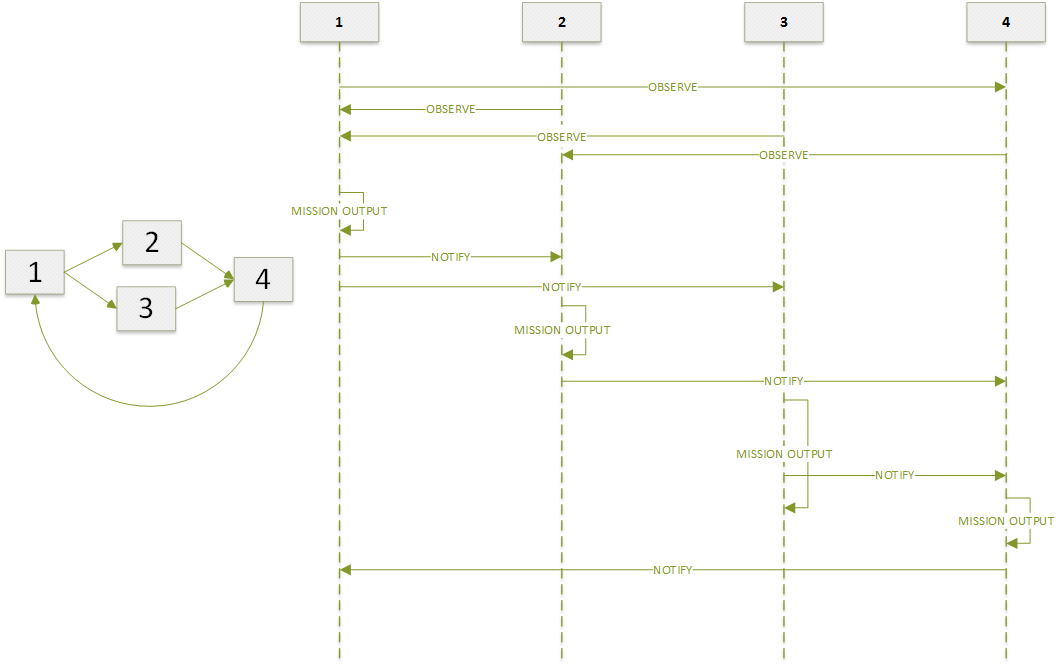
\includegraphics[width=\linewidth]
 {pictures/pub_sub.png}
 \caption{Observer design pattern example}
 \label{fig:observerPattern}
 \end{figure}

In our specific case, we made each declared block of the Graphical Editor both Observer and Observable. 
This means that each block observes another block that comes before it, but at the same time, it is observed by other blocks coming after it.
\\
The change of status consists in the output of the Mission object.
When a block ends to perform its operations, it notifies all its observers passing them the Mission entity.
\\
For example, in figure \ref{fig:observerPattern} the A block observes the D one; the B and C blocks observe the A and the D observes both the B and C.
\\
So, for example, when the A block ends to modify the Mission object it sends it to the B and C blocks at the same time, which are its observers.
\\

The Editor includes a template model of the Main Application, in which almost all the classes are ready to be executed.
\\
However, this template contains several tags that the generation process replaces with specific lines of code, depending on the drawn graph.
\\
The generation process consists in the search for these tags inside the template application. 
The tags are:
\\

\begin{itemize}
\item{\textbf{<dec>}: This tag is the placeholder for the code part where the generator engine puts the declaration and the initialization of the entities represented by each blocks.
}
\item{\textbf{<exe>}: This tag is the placeholder for the code part where the generation process declares the Observer pattern. Here the system defines the observers of each blocks depending on the connections present in the diagram. 
}
\item{\textbf{<tDelay>}: This tag is the placeholder for a boolean attribute. If the diagram includes the Clock block, this tag will be replaced with a "true" value in order to make the Main Application to ask the user for a delay during the Trip definition.
}
\item{\textbf{<mRep>}: This tag is the placeholder for a boolean attribute. If the diagram includes the Mission Repeater block, this tag is replaced with a "true" value in order to make the Main Application ask the user if he wants the Mission to be repeated.
}
\item{\textbf{<tSafe>}: This tag is the placeholder for a boolean attribute. If the diagram includes the Timer Monitor block, this tag is replaced with a "true" value in order to make the Main Application ask the user for a maximum safe time within each Trip must be completed, during the Mission creation phase.
}
\item{\textbf{<tPrt>}: This tag is the placeholder for a boolean attribute. If the diagram includes the Priority Manager block, this tag is replaced with a "true" value in order to make the Main Application ask the user for a priority value during the Trip definition.
}
\item{\textbf{<num>}: This tag is a placeholder for an integer attribute. If the diagram includes the GateFIFO or GateFunnel blocks, this tag is replaced by the number of incoming connections of the related Gate block.
}
\item{\textbf{<act>}: This tag is not replaced by the generation process but we need it in order to indicate the developer where to insert his Custom Action code.
}
\item{\textbf{<eval>}: This tag is not replaced by the generation process but we need them in order to indicate the developer where to insert his custom Evaluator algorithm. 
}
\end{itemize}

\section{Runtime Management}\label{runtimeMng}

The Main Application manages the mission execution with a parallel programming architecture, as shown in figure \ref{fig:threads}.
Indeed when the user starts the execution, the system launches each Mission in a new thread, in order to guarantee a reliable parallel execution.
\\

\begin{figure}[h!]
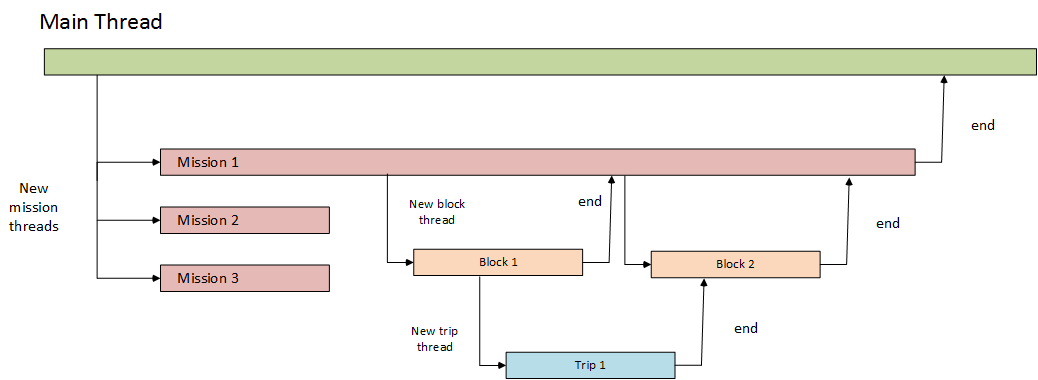
\includegraphics[width=\linewidth]
{pictures/threads.png}
\caption{Example of thread concurrency}
\label{fig:threads}
\end{figure}

Then each mission starts its flow among the blocks, thanks to the Observer design pattern, described in Section \ref{codeGeneration}.
When the mission enters in a new block, the application launches a new thread, in order to run the Mission management code of the block.
We need this new thread because there is the possibility that two or more parallel blocks have to manage the same Mission entity at the same time.
\\

Therefore, when the mission reaches the "Trip Launcher" block, the system starts the execution of the first Trip.
Doing this, it creates a new thread, to manage the trip execution till its end.
\\

As said, each Mission and Trip created by the user have a respective thread that deal with the execution of the entity from the beginning to the end. 
In this way, the blocks that need to monitor these entities can observe the status of the threads, in order to know if the Trip/Mission is still running or is already completed.
\\

It is important to underline that we don't have any synchronization problem among the various threads.
Indeed, there are no dependencies between missions, since each one of them is executed independently from the others.
\\
Inside each Mission entity the trips are executed sequentially:
one trip can start its execution only if the precedent trip in the list has been completed.
\\
Given this independence between missions, the system could dispatch them in a multiple machines cluster.
In this way each Mission can run on a different environment, maximizing the performances and reducing the load of the single machine.
\\

\section{User interface}\label{interface}

Swing is an advanced GUI toolkit. It has a rich set of widgets:
from basic widgets like buttons, labels, scrollbars to advanced like trees and tables. 
Swing itself is written in Java and is part of JFC, Java Foundation Classes: it is a collection of packages for creating full featured desktop applications.
\\

We used the Swing framework to develop the view part of the MVC pattern shown in Section \ref{oomodel},
We needed to develop the three pages of the Pluto Main Application, already described in Section \ref{plutoMainApp}, and we knew that Swing provides all the components that we wanted to put in them.
Indeed, since we used it for the development of many academic projects, we noticed that it allows to build graphical interface in a very fast and easy way.

As an illustrative example, figure \ref{fig:tripsPageStructure} shows the structure of the Trips Page:

 \begin{figure}[h!]
 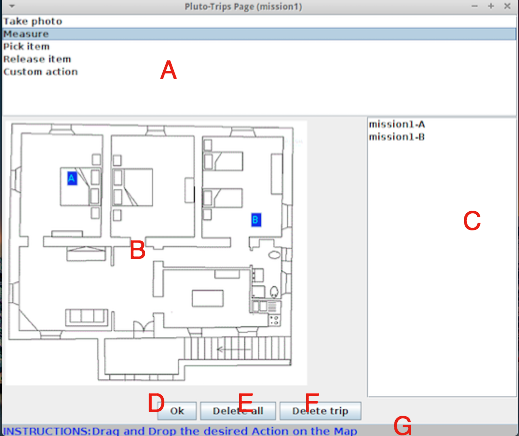
\includegraphics[width=\linewidth]
 {pictures/tripsPageStructure.png}
 \caption{Trips Page structure}
 \label{fig:tripsPageStructure}
 \end{figure}

The Trips Page contains 7 components:

\begin{itemize}
\item {Component A is a \textit{JList}, a list of textual values, in this case the name of the Actions}
\item {Component B is a \textit{JImage}, simply an image representing the Map}
\item {Component C is a \textit{JList}, a list of textual values, in this case the name of the created trips}
\item {Components D,E and F are \textit{JButton}, rectangles that the user can click on}
\item {Component G is a \textit{JTextArea}, an area containing text, in this case the instructions on how to use this page}

All these components are easily usable in Swing, we only needed to import the already provided libraries.
The structure of the other two pages of the Pluto Main Application is very similar to these one, differing only for the contained components.

\end{itemize}


\section{Prototype drone}\label{crazyflie}

For the concrete actuation of the sensing tasks required by each application, we chose the Crazyflie Nano-Quadcopter, shown in figure \ref{fig:crazyflie}.


\begin{figure}[H]
\centering
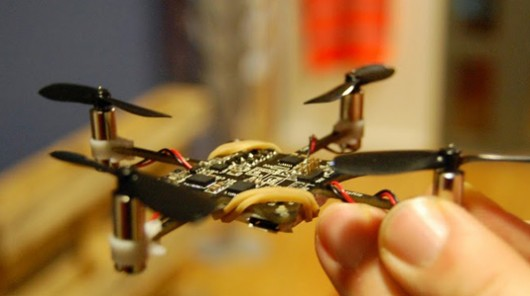
\includegraphics[width=\linewidth]
{pictures/crazyflie.jpg}
  \caption{The Crazyflie Nano-Quadcopter}
  \label{fig:crazyflie}
\end{figure}

The Crazyflie is a tiny quadcopter often referred to as a nano-quad, built using the PCB itself as the frame,developed solely by open source tools. The Crazyflie specs are the following:

\newpage

\begin{itemize}
\item {Small and lightweight, around 19g and about 90mm motor to motor
}
\item {Flight time up to 7 minutes with standard 170mAh Li-Po battery
}
\item {Standard micro-USB connector for charging which takes 20min for the stock 170mAh Li-Po battery
}
\item {On-board low-energy radio@1mW based on the nRF24L01+ chip. Up to 80m range (environment dependent) when using the Crazyradio USB dongle}
\item{Radio bootloader which enables wireless update of the firmware
}
\item{Powerful 32 bit MCU: STM32F103CB @ 72 MHz (128kb flash, 20kb RAM)
}
\item{3-axis high-performance MEMs gyros with 3-axis accelerometer: Invensense MPU-6050
}
\item{Available footprints to manually solder magnetometer HMC5883L/HMC5983 or/and barometer MS5611
}
\item{4-layer low noise PCB design with separate voltage regulators for digital and analog supply
}
\end{itemize}

We use a particular API that makes the drone move from a \textit{startingLocation} to a \textit{destination} in the environment:
\\

\begin{lstlisting}
	move(startingLocation, destination)
\end{lstlisting}

To concretely control the Crazyflie, there is a Python library which gives high level functions and hides the details.
The precedent API uses the following to send the control commands to the Crazyflie:

\begin{lstlisting}
	send_setpoint(roll, pitch, yaw, thrust)
\end{lstlisting}

The arguments roll/pitch/yaw/trust is the new set-points that should be sent to the copter.
For example, to send a new control set-point:
\\

\begin{lstlisting}
	roll    = 0.0
    pitch   = 0.0
    yawrate = 0
    thrust  = 0
    crazyflie.commander.send_setpoint(roll, pitch, yawrate, thrust)
\end{lstlisting}

Changing the \textit{roll} and \textit{pitch} will make the quadcopter tilt to the sides and thus change the direction that it's moving in.
Changing the \textit{yaw} will make the quadcopter spin.
The thrust is used to control the altitude of the quadcopter.

By dynamically adjusting these four parameters we can make the Crazyflies move to the locations specified by the user through the Pluto User Interface.
\chapter{Evaluation}
\label{cap6}


\section{Applicability of the Pluto framework}\label{applicability}


We developed our programming framework thinking about indoor applications utilizing nano-drones; actually, since we work at a sufficiently high level of abstraction, because we can use an API which can make the drones navigate in the environment, the model can be extended to almost every kind of drone, aerial terrestrial and aquatic.
So, we can say that the Pluto programming framework is "drone independent", and this greatly extends its applicability, including also outdoor, aquatic and terrestrial environments; it is in charge of the programmer to manage the interaction between Pluto and the specific type of drone he wants to use for the particular application he's developing.

Pluto is fully exploited when there is a team of drones to manage (see \ref{fig:WIS} and \ref{fig:DD}), although it perfectly works also in the case of a single drone (see \ref{fig:OF}).

Since we decided to use a Team-level approach (see \ref{teamlevel}), our model can be used for developing applications where the user can give to the system a set of actions to be performed; the dispatching of these actions is managed by the "central brain", which takes care of assigning the drones to the action and to handle all the exceptions (battery low, crashes etc.). So, the drones are only actuators that perform an action, there is no communication between them, their behavior is monitored and decided by the central brain.

Since drones cannot communicate between them, Pluto cannot be used for applications where drones must perform some kind of action requiring explicit communication or data exchange between them; the logic is managed by the central brain, so communication between drones is always mediated by this component; a drone can send data to the central brain, and this could send again that data to another drone.

Hereinafter we analyzed some already existing example applications, showing whether they can be managed/developed with the Pluto programming framework or not.

\subsection{Alfalfa Crop Monitoring and Pollination}\label{alfalfa}

The Alfalfa Crop Monitoring and Pollination\cite{alfalfa} is a typical example of swarm-level approach application.
Alfalfa is an important food crop for cattle and requires an external pollinator (e.g. bees) to produce seeds. In recent years, colony collapse disorder has devastated honeybee populations and jeopardized the cultivation of important crops.
A swarm of drones can pollinate the alfalfa plants and also monitor them for pests and diseases, trough visual spot checks.
So, the whole application provide three periodic actions: searching for pests, searching for diseases, and looking for flowers in bloom.
Each one of these actions is achieved by taking pictures of the plants.
The user may need to define time constraints within the pollination  action must be completed.

The following Pluto Editor graph describes the Alfalfa Crop Monitoring and Pollination\cite{alfalfa} application:

\begin{figure}[H]
  \centering
  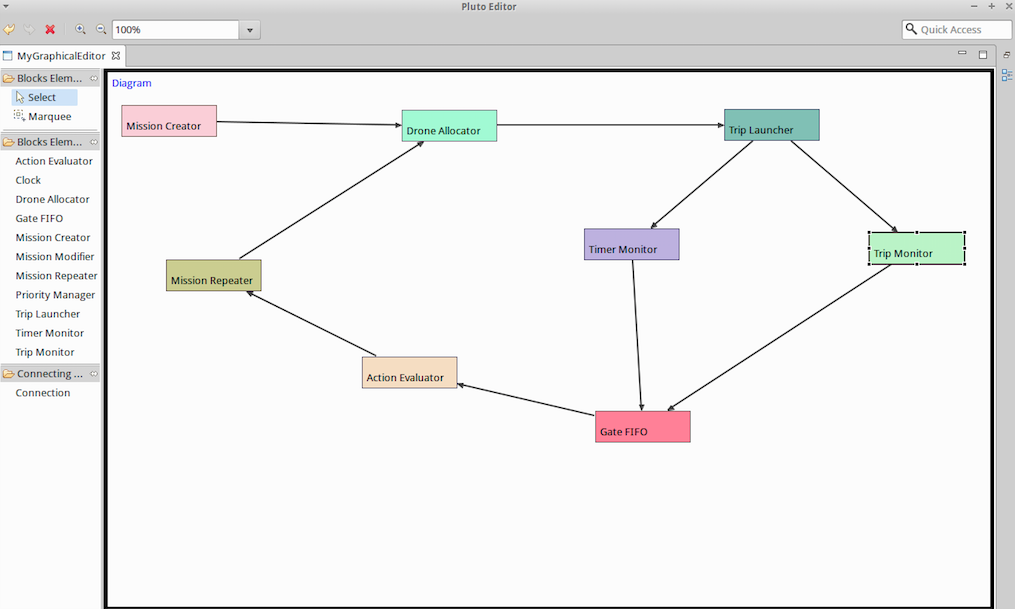
\includegraphics[width=\linewidth]{pictures/alfalfaEditor.png}
  \caption{Pluto graph for the Alfalfa Crop Monitoring and Pollination application}
  \label{fig:alfalfaGraph}
\end{figure}


We tried to implement this application drawing a diagram showed in figure \ref{fig:alfalfaGraph}. this diagram is an extension of the basic one showed in the chapter \ref{descriprionOfModel}. In order to satisfy the application constraints, we needed to add a couple of new blocks. The first difference consist in the presence of the TimerMonitor block parallel to the TripMonitor. This block is added in parallel because we need it to monitor the running Trip at the same time of the TripMonitor. Then the GateFIFO will wait for the first instance of the Mission from one of these two blocks. After that, if the mission is completed, it will pass through the MissionEvaluator that will evaluate the actions done. Further the MissionRepeater will make the mission to start again from the first Trip. With these blocks we were able to respect the main constraints of the Alfalfa\cite{alfalfa} application. After the generation of the code from the diagram, we needed to make some customizations in the Main Application sources, such as the add of a Pollination Action and the implementation of the Evaluator algorithm. Following there are these two pieces of code commented to better understand their behaviors.

\begin{lstlisting}
		String result = null;

		// Retrieve all entries of the map
		for (Map.Entry<Trip, Object> entry : dataMap.entrySet()) {

			// consider only the trips related to the mission to evaluate
			if (missionToEvaluate.getCompletedTrips().contains(entry.getKey())) {
				
				// take the Photo of the current Trip iteration
				Photo photo = (Photo) entry.getValue();
				
				// checking pest and disease
				if (photo.hasPest() || photo.hasDisease())
					
					return "WARNING: Pest/disease at location: "
							+ entry.getKey().getTargetLocation();

				// checking for some bloom
				if (photo.hasBloom()) {

					// create a new Trip to pollinate the flowers
					Trip trip = new Trip();
					trip.setName("PollinateTrip");
					trip.setTargetLocation(entry.getKey().getTargetLocation());
					trip.setAction(Action.POLLINATE);
					trip.setStatus(Trip.WAITING);

					// add this new trip to the list of the mission
					missionToEvaluate.getTrips().add(trip);
					// set the mission status to STANDBY
					missionToEvaluate.setStatus(Mission.STANDBY);
				}
			}
		}

		// set the result of the evaluation
		result = "Success";
		return result;
\end{lstlisting}

The "dataMap" attribute is an \textit{hashmap} that binds each Trip with the picture taken by the action.
For each photo taken by the drone, the code checks the presence of \textit{pests} and \textit{diseases}. In that case, the system will warn the farmer the location where the problem exists, through the log function.
If there are \textit{blooms}, the plants at that location must be pollinated, so a new Trip is created: its status is set to WAITING, its Action is set to Pollinate and the target location is set to the same location of the Trip that found the bloom.
Finally this Trip is added to the execution queue of the mission. The Mission status is set to STANDBY because there is something new to do.
\\

The following is possible source code of the Pollination Action.

\begin{lstlisting}
	// This is the method called by the drone
	// after it reaches the target location
	@Override
	public Object doAction() {
		Camera camera = System.getCamera();
		Photo photo = camera.takePhoto();
		return photo;
	}
\end{lstlisting}

In the end we simulated the final user, so we created two missions with eight trips each, as if we needed to monitor a real field.

\begin{figure}[H]
  \centering
  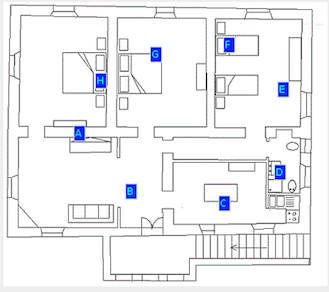
\includegraphics[width=\linewidth]{pictures/area3.png}
  \caption{Trip distribution screenshot}
  \label{fig:alfalfaArea}
\end{figure}

To further understand the behavior of the MainApplication we drawn a sequence diagram, showed in figure \ref{fig:alfalfaSequence}.

\begin{figure}[H]
  \centering
  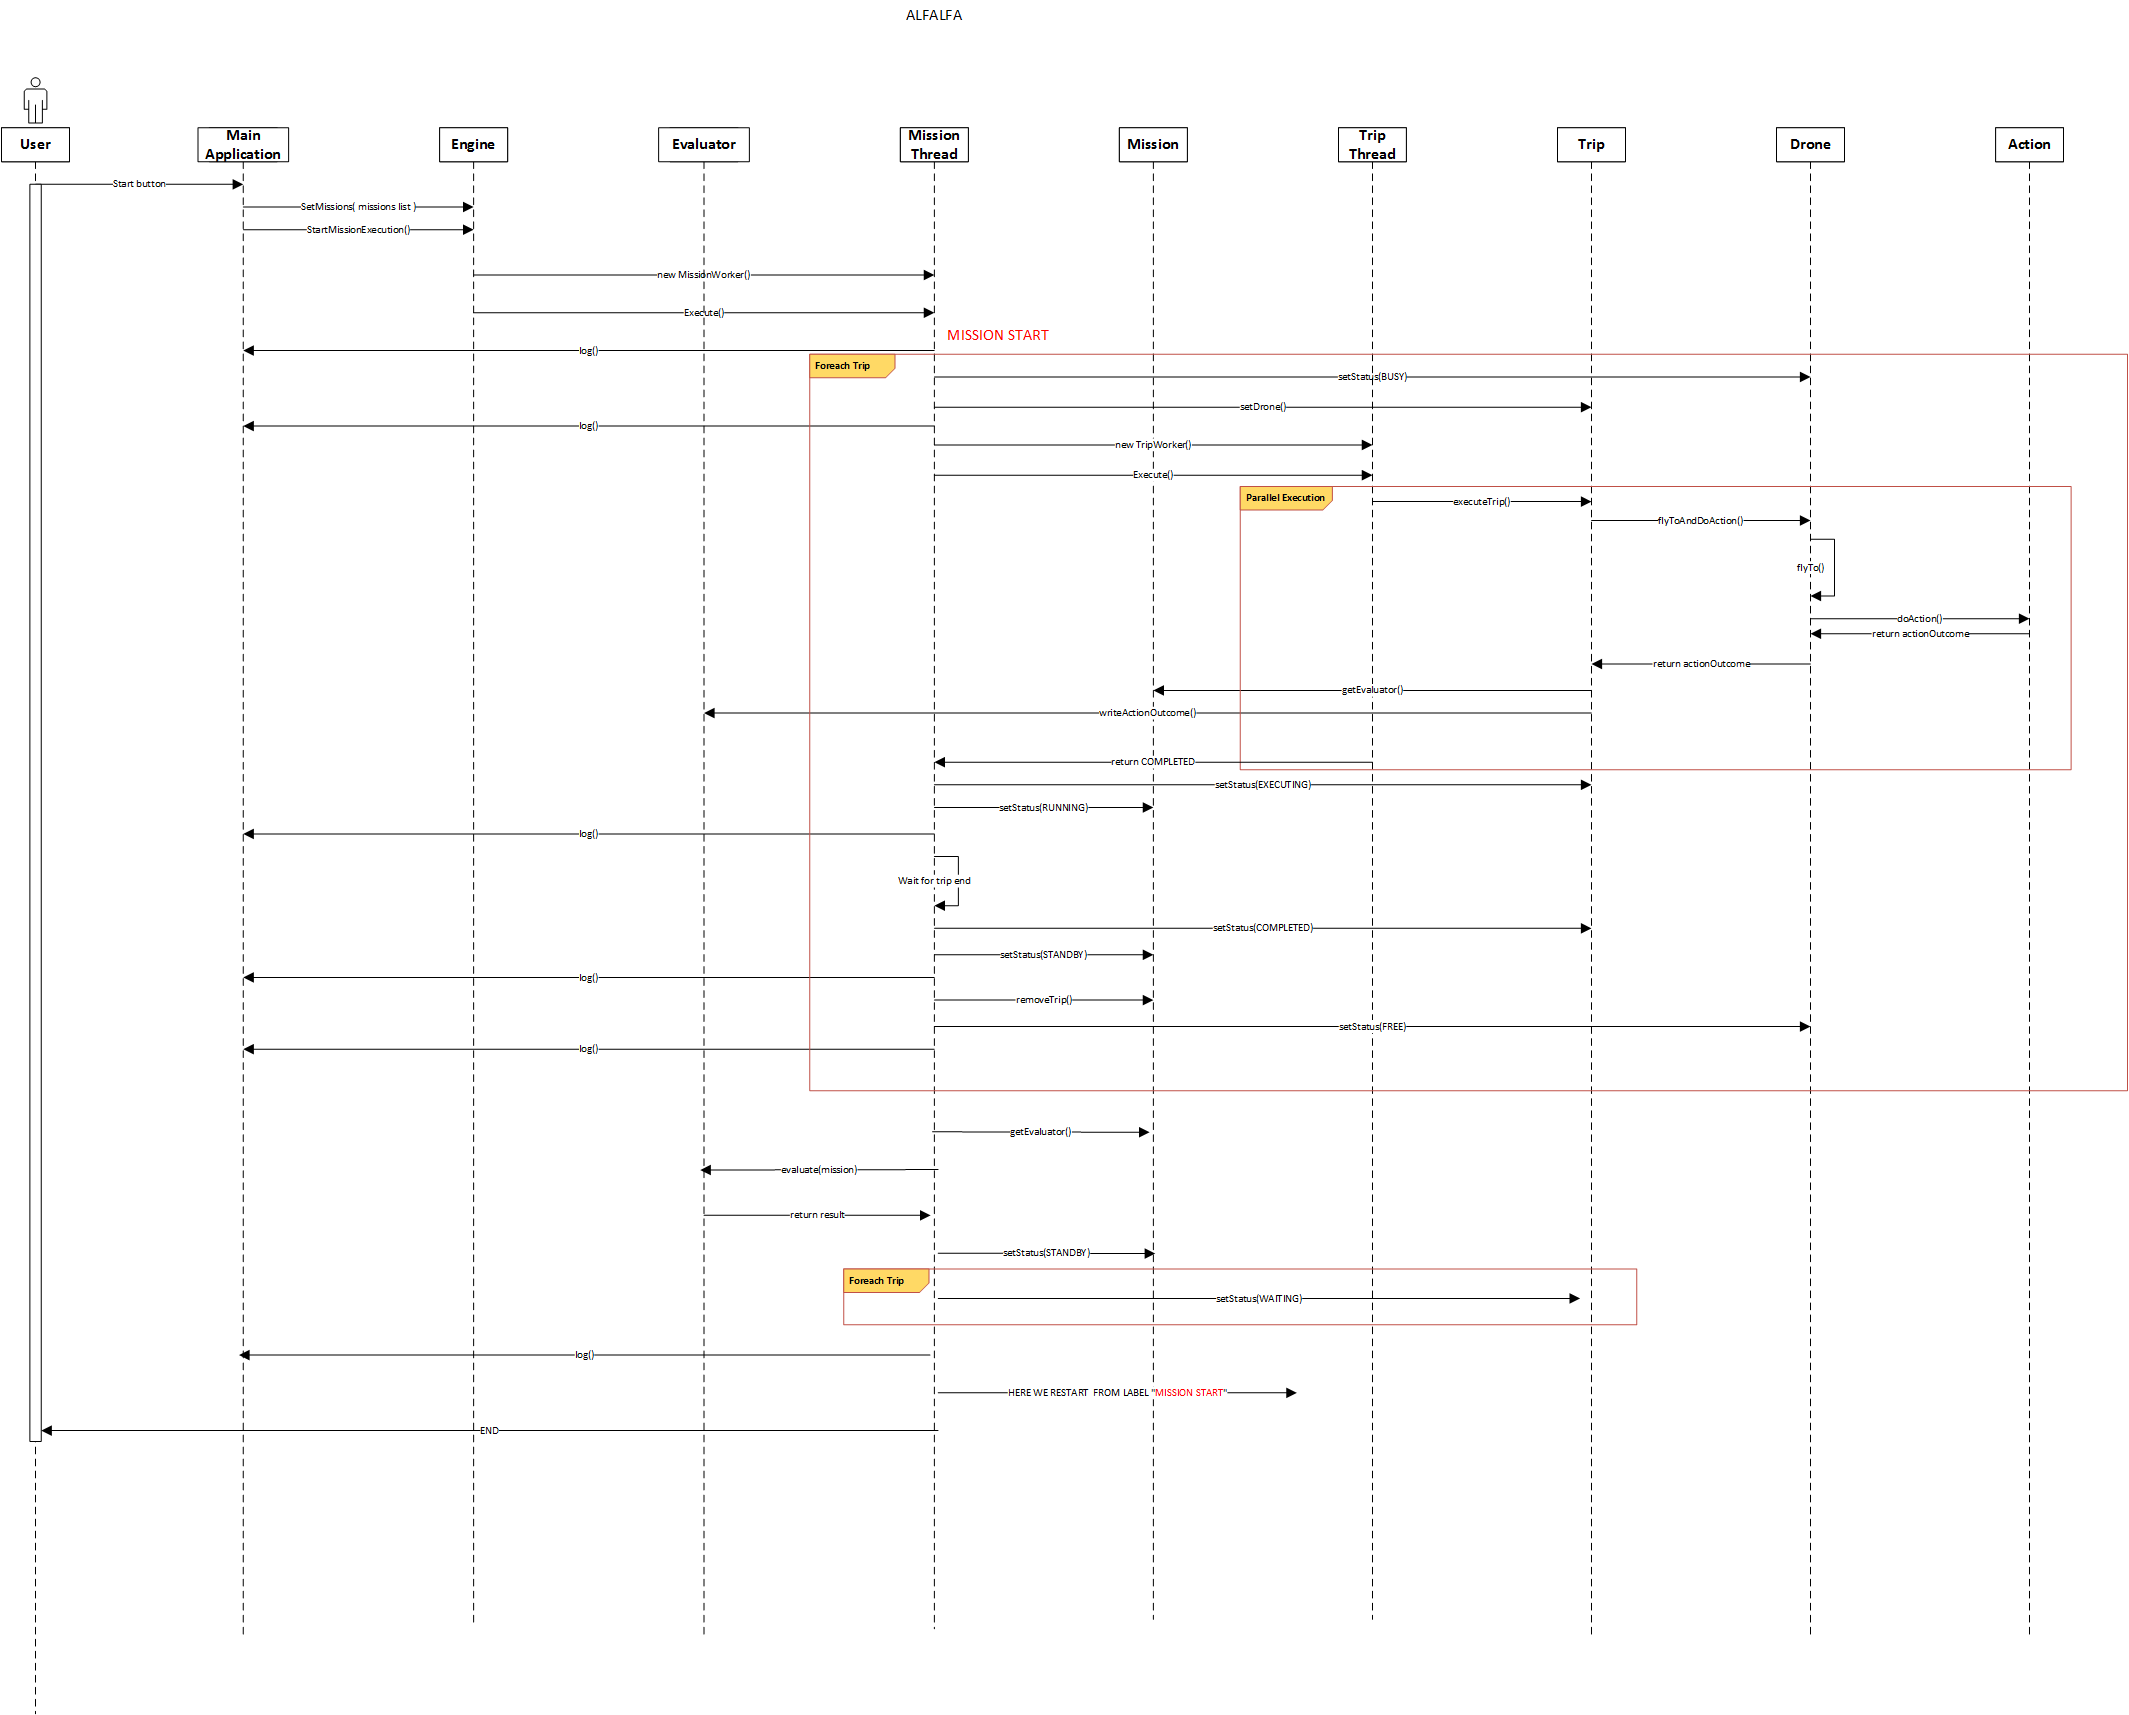
\includegraphics[width=\linewidth]{pictures/Alfalfa_Sequence.png}
  \caption{Sequence diagram of the MainApplication behavior}
  \label{fig:alfalfaSequence}
\end{figure}

\subsection{Aerial mapping of archaeological sites}\label{aerialMapping}

This application allows archaeologists to survey ancient sites without involving their direct presence on it.
Many Ortophotos of the site are taken, so that the archaeologists can see the geometric layout of the site, without physically walking near it, which could cause irreparable damages.
An orthophoto is an aerial photo that is geometrically-corrected so that distances between pixels are proportional to true distances, such that the photo can be used as a map.
Drones are sent to take a series of ortophotos which then will be stitched together to derive a single ortophoto; if the individual pictures do not have sufficient overlap, the resulting orthophoto will show excessive aberrations, and, in that case, the drone is sent out again to take more pictures.
If the obtained ortophoto is not adequate, the archaeologists should be able to send more drones on that particular area.
The drones must perform their actions in a limited amount of time, since if too much time pass between two ortophotos, the scene may change.

The following figure is the Pluto editor graph needed to create the Aerial Mapping of the "Domus dei Putti Danzanti" site application. 

\begin{figure}[H]
  \centering
  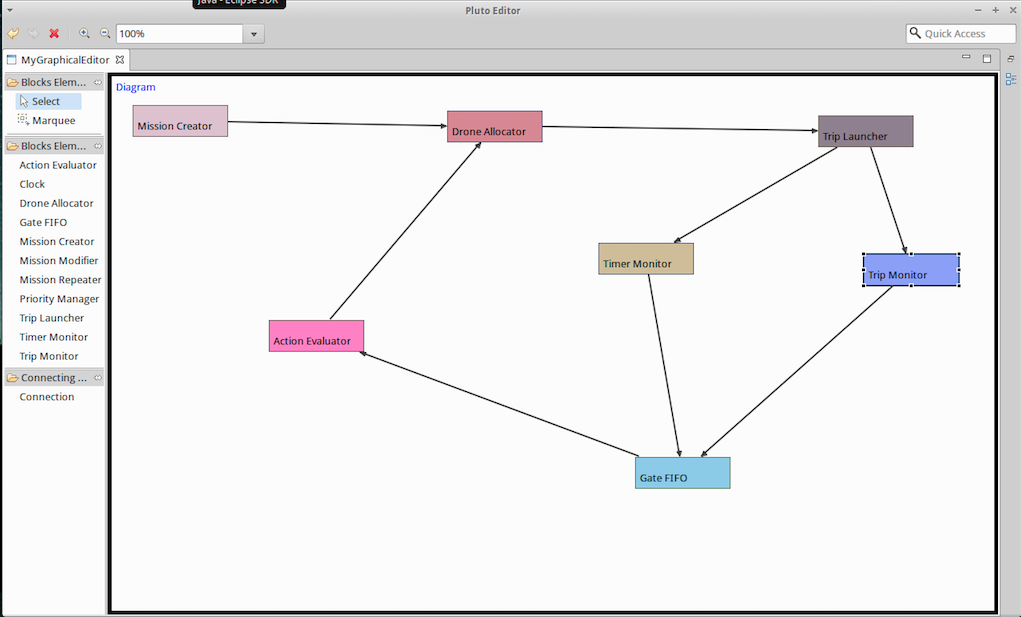
\includegraphics[width=\linewidth, height=8cm]{pictures/puttiEditor.png}
  \caption{Pluto graph for the Aerial Mapping of the "Domus dei Putti Danzanti" site}
  \label{fig:puttiGraph}
\end{figure}

The drones can already take pictures thanks to the \textit{Take Photo} action.
To send the drones to take pictures over the site location, the user has to simply create the Missions entities and add the Trips to the map he will be provided with.
In the case the archaeologists want to send more drones on the locations where they can't obtain an adequate ortophoto, they just have to add more Mission entities.
For example, if one archaeologist want to send 3 drones on a particular location, he has to create 3 Mission entities.
Then for each Mission he simply  has to drag and drop the \textit{Take photo} action on that particular location.
The GateFIFO block takes as input two Mission instances, one from the Trip Monitor block and the other one from the Timer Monitor.
It takes care of propagating only the first instance that arrives to it.
For example, if the timer has expired then it will propagate the Timer Monitor instance, otherwise the Trip Monitor one.
Thanks to the ActionEvaluator block, that analyzes the drones data at the end of the missions, the Main Application can decide if the photos are good enough or if more drones must be sent out to take new pictures in that specific location.
It is important to underline that, using the Pluto framework, it is not possible to obtain the very same behavior of the original application.
Indeed, two consecutive photos must be taken within a time constraint.
This cannot be fulfilled with Pluto, since the Timer Monitor block deals with a time interval that starts when the drone leaves the base station, ensuring that it will take the picture before the time interval expires.
So, there is no way to state a time constraint between two consecutive photos.


Concerning the code of the Evaluator block needed for the development of the Aerial Mapping\cite{putti} application, as for the previous application, we can find each photo taken during the missions in the "dataMap" parameter, that is an hashmap that create a relation between a Trip and the photo taken through its Action.
First of all, the ortophotos are stitched together to obtain the final ortophoto, trough the \textit{stitch} function.
If the final ortophoto shows excessive aberration, the ortophotos composing it are analyzed and if they don't have sufficient overlap, few new Trips are created with the same target locations of the photos to be taken again. 
The Mission status is set to STANDBY because there is at least a new inserted Trip to execute.
It is important to underline that this application differs from the Alfalfa\cite{alfalfa} one, because the Evaluator algorithm acts in a different way: in Alfalfa\cite{alfalfa} application the algorithm takes care of analyzing the photos of a single mission without considering the others; now, instead, the evaluation needs to merge all the photos of every missions to calculate the aberration. This is why, as said in section \ref{blocks}, we decided to activate the ActionEvaluator block only when the Mission status is Completed. 
Following we show our implementation for the Evaluator algorithm:
\\
\begin{lstlisting}
		String result = null;
		// generate the final ortophoto
		OrtoPhoto ortophoto = stitch(dataMap.values());
		
		// if the aberration is greater than a fixed threshold
		if(ortophoto.getAberration() > ABERRATION_THRESHOLD){
			
			// for each photo that compose the ortophoto
			for (Photo photo: ortophoto.getPhotoCollection()){
				
				// if the overlap of the photo is not enough
				if (ortophoto.getOverlapOfGivenPhoto(photo) < OVERLAP_THRESHOLD){
					
					// Retrieve all entries of the map
					for (Map.Entry<Trip, Object> entry : dataMap.entrySet()) {
						
						// take the Photo of the current iteration
						Photo p = (Photo) entry.getValue();
						
						// if we found the photo in the map
						if(photo.equals(p)){
							
							// create a new Trip
							Trip trip = new Trip();
							trip.setName("NewTrip");
							trip.setTargetLocation(entry.getKey().getTargetLocation());
							trip.setAction(Action.TAKE_PHOTO);
							trip.setStatus(Trip.WAITING);

							// add this new trip to the list of the mission
							missionToEvaluate.getTrips().add(trip);
							
							// set the mission status to STANDBY
							missionToEvaluate.setStatus(Mission.STANDBY);
						}
					}		
				}
			}
		}
        
        // set the result of the evaluation
		result = "Success";
		return result;
\end{lstlisting}

In order to show the real runtime execution of the Aerial Mapping application with Pluto, we now show a real scenario:
there are 7 drones and 1 big area to monitor, and we want to send all the drones in that area at the same time to take the ortophotos.
As usual, the user has to create 7 Mission entities.
Then, for each Mission, he has to create the list of Trips by using the map to drag and drop the action \textit{Take photo} on the locations forming the big area.



\subsection{PM10}

The PM10\cite{pm10} application is used to build 3D maps of pollution concentration in the atmosphere. 
Initially, there is a predefined 3D grid over which drones are sent to sample the quantity of pollution.
So the drones build a spatial profile of pollution concentration and compute gradients among the areas of higher concentration.
Finally the drones are sent along this gradients to sample the pollution concentration, in order to improve the spatial profile representation.
Any two consecutive samples must be gathered within a given time bound, otherwise the system will take care of speeding up the execution.

The following figure is the Pluto editor graph needed to create the PM10 application:

\begin{figure}[H]
  \centering
  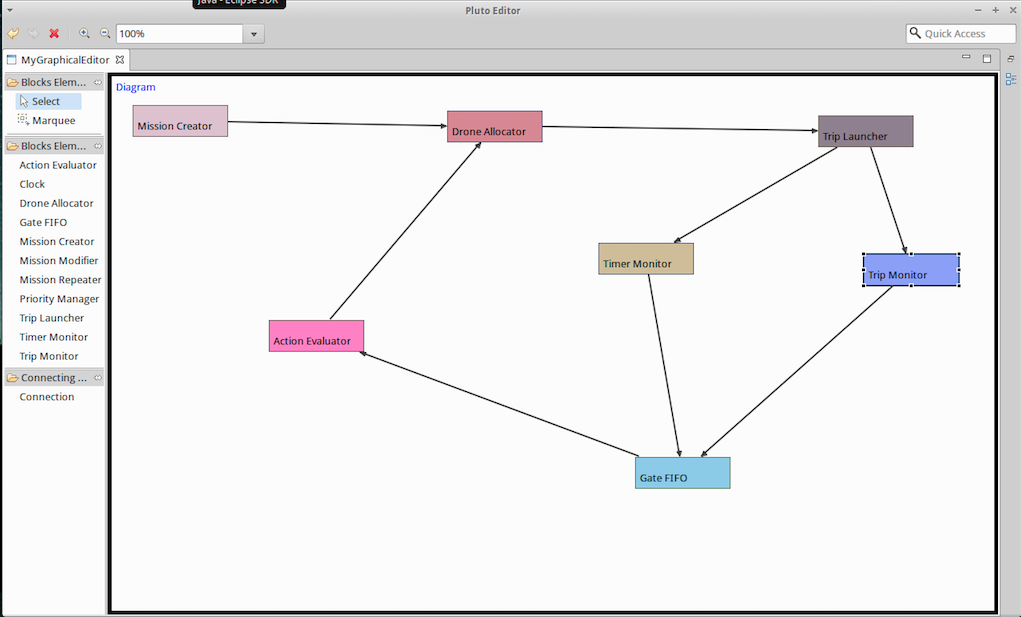
\includegraphics[width=\linewidth]{pictures/puttiEditor.png}
  \caption{Pluto graph for the PM10 application}
  \label{fig:pm10Graph}
\end{figure}


For the measurements of pollution quantity, the \textit{measure} action can be used.
The spatial grid must be manually built by the user, organizing the Trips of each Mission on the map he's provided with.
The data collected by the drones are not photos anymore, but a \textit{pollutionQuantity} value which indicates the percentage of pollution in that area.
Then, thanks to the MissionEvaluator blocks, the \textit{pollutionQuantity} variables are confronted and the gradients between areas of higher concentration are computed.
Then the drones will be sent along this gradients, improving the spatial profile.
As for the Aerial Mapping application, shown in section \ref{aerialMapping}, Pluto cannot fulfill the time constraint between two consecutive pollution samples.
As already explained, the timer of Pluto starts when the drone leaves the base station and ensures that it will perform the action within that time interval, but there is no way to constrain the time between two consecutive samples.
The GateFIFO block takes as input two Mission instances, one from the Trip Monitor block and the other one from the Timer Monitor.
It takes care of propagating only the first instance that arrives to it.
For example, if the timer has expired then it will propagate the Timer Monitor instance, otherwise the Trip Monitor one.

Below there is our implementation of a possible Mission Evaluator algorithm:
\\

\begin{lstlisting}
		String result = null;

		// building a new map with only the trip-measure couples of the mission
		// to evaluate
		Map<Trip, Integer> missionMap = new Map<Trip, Integer>();
		for (Map.Entry<Trip, Object> entry : dataMap.entrySet()) {
			if (missionToEvaluate.getCompletedTrips().contains(entry.getKey())) {
				missionMap.put(entry.getKey(), (Integer) entry.getValue());
			}
		}

		// this method use the Trip location and the pollution measure to
		// calculate
		// the gradients and then return a list of String that indicates
		// the positions of these gradients
		List<String> gradientsPositions = calculateGradients(missionMap);

		for (String position : gradientsPositions) {

			// create a new Trip to calculate pollution at the gradient position
			Trip trip = new Trip();
			trip.setName("GradientTrip");
			trip.setTargetLocation(position);
			trip.setAction(Action.MEASURE);
			trip.setStatus(Trip.WAITING);

			// add this new trip to the list of the mission
			missionToEvaluate.getTrips().add(trip);
			// set the mission status to STANDBY
			missionToEvaluate.setStatus(Mission.STANDBY);
			
		}
			
		// set the result of the evaluation
		result = "Success";
		return result;
\end{lstlisting}


Now we show the execution of the PM10 application with Pluto in a particular scenario:


\subsection{PURSUE}


The PURSUE application\cite{pursue} is representative of surveillance applications. A team of drones monitor an area and they have to follow moving objects which pass through, taking a picture of each one of them when they enter in the camera field.
To do so, drones can operate in two distinct modes: when in "patrolling mode" they simply inspect an area, while when an object is found they switch to "pursuing mode" and start to follow the object.
Since an object could move faster than the drones, no drone can follow it constantly, the system must take care of switching between the real drones in order to constantly follow the target.
There are time constraints to respect between the detection of a moving object and when its picture is taken and, in case of violations,every tracked object with at least one acquired picture is released from tracking, to regain the drone resources and lower the acquisition latency for the next object.
\\

The PURSUE application represents a limit for the Pluto programming framework.
Indeed, in our model, the drones perform their action only at the end of the Trip, so it's not possible for them to immediately take a picture of the moving object.
This problem can be lowered by inserting a lot of trips in the area to monitor, with strict time constraints on them.
But still there is no way for the drones to actively follow the moving objects.


\newpage

All the previous applications were already developed and tested with other systems, like Karma\cite{karma} and Voltron\cite{voltron}, but we also developed new applications and tested our framework on them, the Object-finder (OF), the Warehouse item-finder (WIF)and the Drugs distribution(DD); in the following subsections we will describe these applications in details, also using a visual representation of their behaviour, and sequence diagrams, to make understand better the whole functioning of each one of them.

\subsection{Object-finder (OF)}

This application will help users to find various objects, in a domestic fashion, like shoes, keys, books etc:

\begin{itemize}
\itemsep2pt
\item{
the user decides which item wants the drones to look for and the area to be inspected
}
\item{
the main system organizes the team of drones, deciding the path for each one of them
}
\item{
the drones fly to the assigned location and, if found, bring the object back to the user, through a magnet or robotic arm
}
\end{itemize}


\begin{figure}[H]
  \centering
  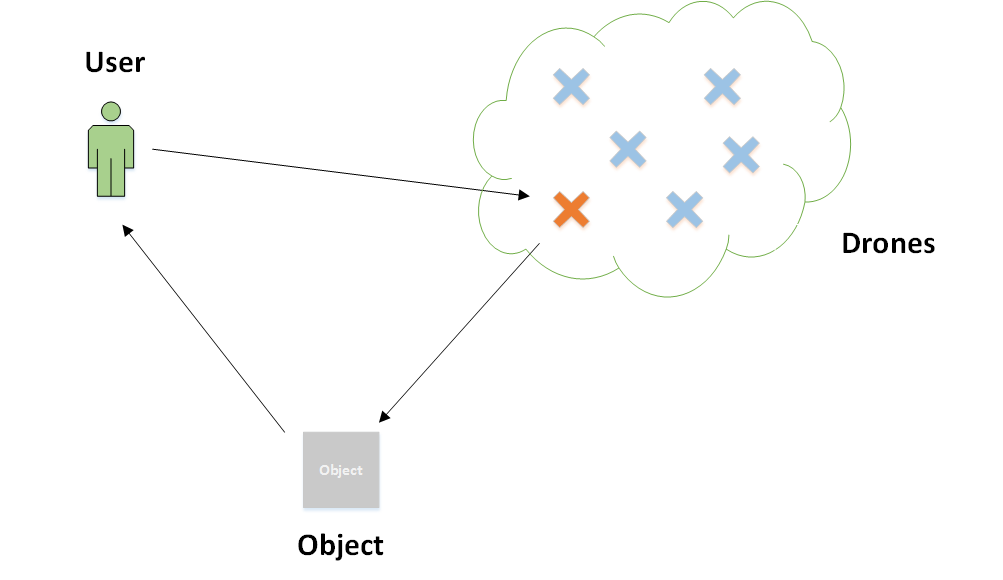
\includegraphics[width=\linewidth]{pictures/OF.png}
  \caption{The basic functioning of the Object-finder application}
  \label{fig:OF}
\end{figure}


\begin{figure}[H]
  \centering
  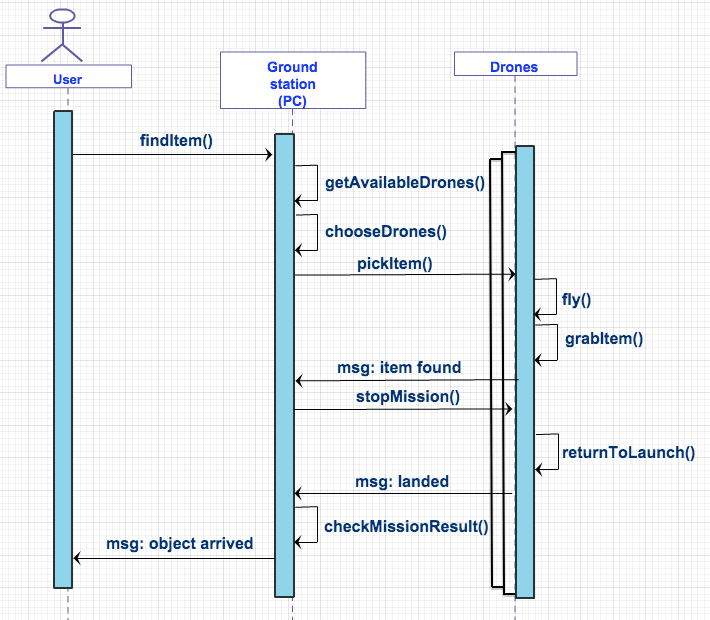
\includegraphics[width=\linewidth, height=8cm]{pictures/OF_sequence.png}
    \caption{Sequence diagram of the Object-finder application}
  \label{fig:OFSequence}
\end{figure}


The user sets which item he needs in the ground station and sends the command; the ground station checks if there are drones unavailable, maybe broken or with low battery status. Then selects the drones that could carry out the mission and send them the command to start the mission. The ground station communicate with each drone, but in the sequence diagram we described the communication only with one of them. After the mission starts, all the drones start looking for the item in the house and when the lucky one finds it, it grabs it and send a notification message to the Ground Station. So, the Ground Station sends a “Stop Mission” message to each drone flying; in this way they could return to the home position. In the end the Ground Station checks if the drone with the item is returned and notifies it to the user.

\newpage

\subsection{Warehouse item-finder (WIF)}

This application will be used to manage a warehouse, taking a list of objects to the user:

\begin{itemize}
\itemsep2pt
\item{
the user makes a list of needed items and writes it on his laptop, tablet or smartphone}
\item{
the main system organizes the swarm of drones and decide which one will take each item in the list
}
\item{
the drones fly to the assigned object and bring them back to the user, through a magnet or robotic arm
}

\end{itemize}


\begin{figure}[H]
  \centering
  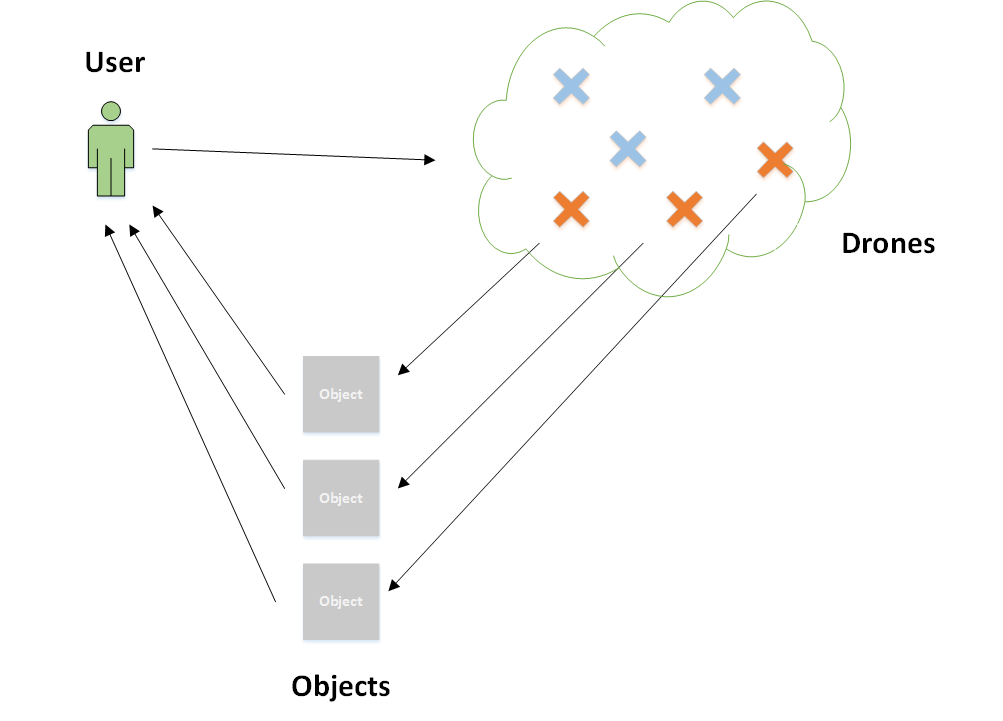
\includegraphics[width=\linewidth]{pictures/WIF.png}
  \caption{The basic functioning of the Warehouse item-finder application}
  \label{fig:WIS}
\end{figure}


\begin{figure}[H]
  \centering
  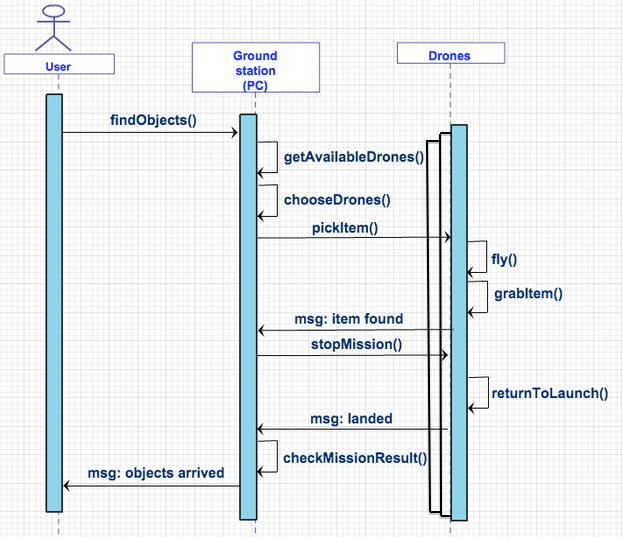
\includegraphics[width=\linewidth, height=8cm]{pictures/WIF_sequence.png}
    \caption{Sequence diagram of the Warehouse item-finder application}
  \label{fig:WISSequence}
\end{figure}

\newpage

\subsection{Drugs distribution (DD)}\label{dd}

This application is thought to assist elders to take their daily drugs, in an hospice context:

\begin{itemize}
\itemsep2pt
\item{
the nurse will prepare a little box with each patient’s daily medicine
}
\item{
each drone, at the right time of the day, will bring the box to his assigned patient
}
\item{
after carrying out their action, the drones return to the start location
}

\end{itemize}


\begin{figure}[H]
  \centering
  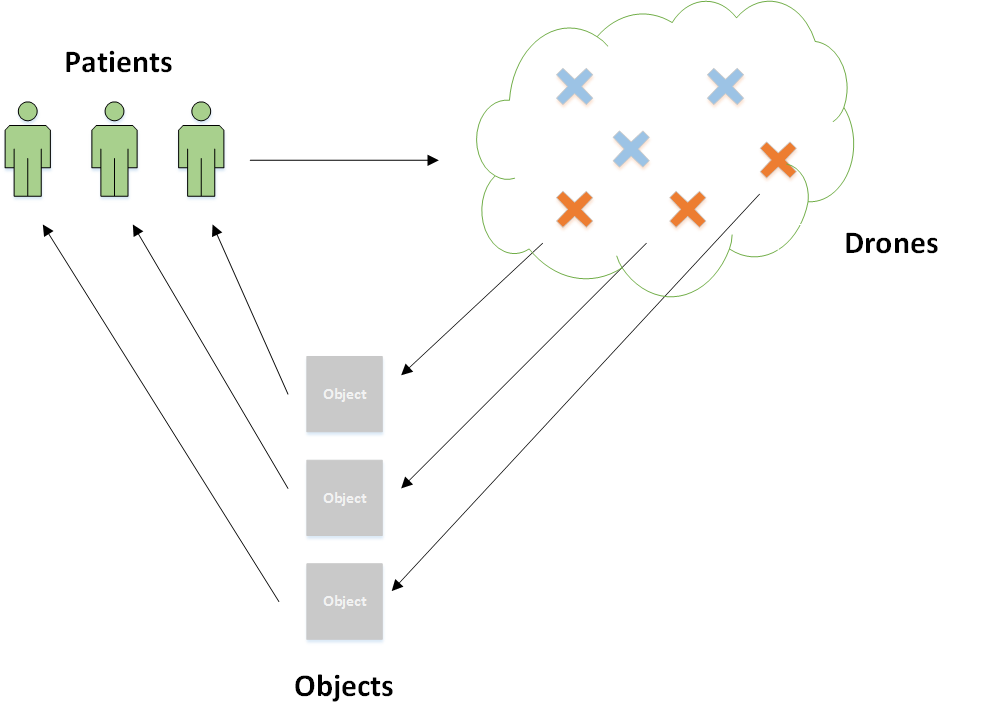
\includegraphics[width=\linewidth]{pictures/DD.png}
  \caption{The basic functioning of the Drugs distribution application}
  \label{fig:DD}
\end{figure}


\begin{figure}[H]
  \centering
  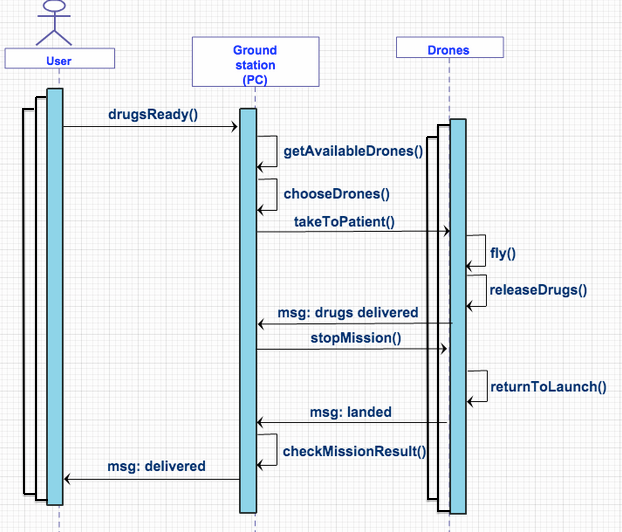
\includegraphics[width=\linewidth,height=8cm]{pictures/DD_sequence.png}
\caption{Sequence diagram of the Warehouse Drugs-distribution application}
  \label{fig:DDSequence}
\end{figure}



The OF,WIF and DD applications can be easily developed with the Pluto editor.
Their basic versions are represented by the basic graph of each application, shown in figure (see \ref{fig:firstStep}),and they can be possibly enriched with the Priority Manager and Timer Monitor blocks, in order to improve the priority of the failed trips or to give a time constraint within the trips must be executed.

\newpage

\section{Usability of the model}
\label{usability}

To evaluate the concrete usability of the Pluto programming framework, we decided to test it on real people, proposing them two "exercises".
The tester were recruited in the "Politecnico di Milano" and "SICS Swedish ICT" environment, in order to guarantee a solid development background and to avoid possible lack of programming knowledge.
We created one exercise for each component of Pluto framework.
The first one consists in the development of an application using the Pluto Graphical Editor.
The exercise is split in three levels, starting from a very basic version and going through more difficult versions. Each version asks the user to add a new functionality by using the available components in the Editor.
The second exercise, instead, asks the user to use the generated code from the previous exercise to run the Pluto Main Application, then asks to create some missions and, in the end, to run them.
The application we choose for the exercises is the Drugs Distribution, already described in section \ref{dd}, because it's very suitable for the type of evaluation we want to perform.
Indeed its basic version can be extended with many features, for example using the Mission Modifier block (section \ref{mm}), and this is exactly our purpose.
The results are shown in section \ref{surveyResult}.
After the execution of the exercises, we asked the users to leave a feedback, proposing them a survey, built according to some metrics that we have defined and that we describe in section \ref{survey}.

\subsection{Proposed exercises}
\label{exercise}

We give the user a complete and sound explanation of the Pluto programming framework, showing how the graphical editor works (shown in section \ref{plutoGraphicalEditor}) and giving him the list of the available entities (shown in section \ref{entities}) and of the implemented blocks (shown in section \ref{blocks}), together with an explanation of the meaning and functionality of each one.
The same explanations are given for all the components of the Pluto User Application (shown in section \ref{plutoMainApp}).

\subsubsection{First Exercise}

The exercise proposes the development of the Drugs Distribution application (shown in section \ref{dd}) in three different versions, increasingly harder to implement:

\begin{itemize}
\itemsep2pt
\item{
\textit{basic version}: we ask the user to implement the basic version of the Drugs Distribution application
}
\item{
\textit{medium version}: we ask the user to raise the priority of the failed trips and to re-insert them in the queue of next trips to be launched, and to add a delay for the trips.
}
\item{
\textit{hard version}: we ask the user to add a time constraint within each trip must be completed, that is the same feature implemented by the Timer Monitor block, but using the Mission Modifier block.
}
\end{itemize}

To solve the first part of the exercise, the user has to create the graph shown in figure \ref{fig:firstStep}, that represents the very basic scheme of each application, since it uses only the basic blocks.
Once created the graph, the user has to right click on the panel and choose "generate code" to accomplish the first step of the exercise.
This is a very easy task to perform, but we think it's useful, because make the user confident with the basic features of Pluto, such as the basic blocks and the code generation mechanism.


\begin{figure}[htb]
  \centering
  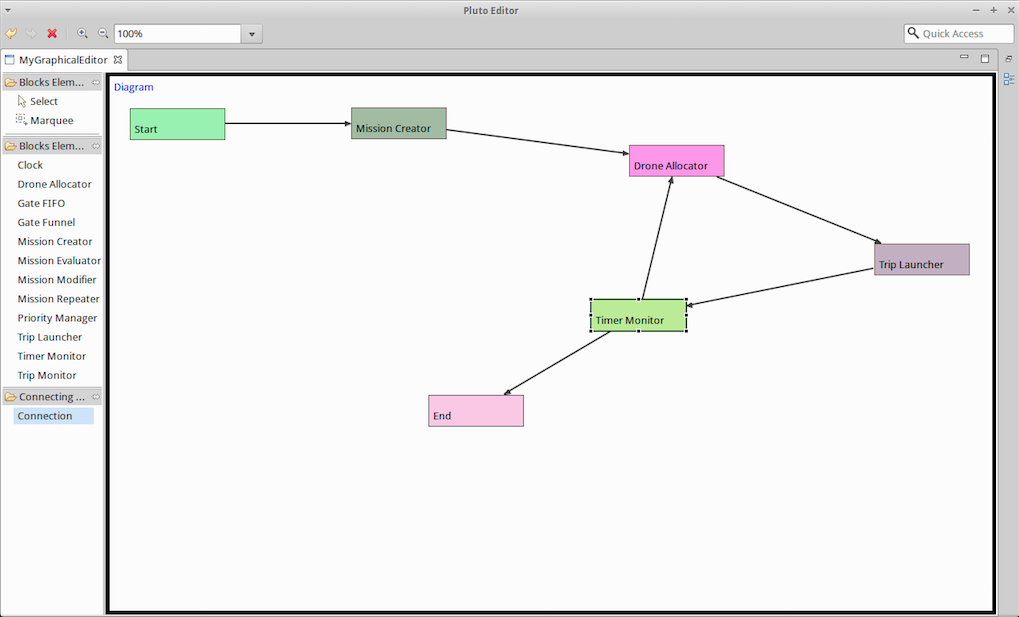
\includegraphics[width=\linewidth]{pictures/EditorScreen.png}
  \caption{Solution of the first step}
  \label{fig:firstStep}
\end{figure}

\newpage

To solve the first part of the second step of the exercise, the user has only to understand that the functionality to add is already implemented by the Priority Manager block, so he has only to add this block to the graph in the right point.
Since we ask him to re-insert the failed trips in the queue of unexecuted trips he has to put the block between the Trip Monitor and the Drone Allocator, as shown in figure \ref{fig:secondStepPriority}.

\begin{figure}[htb]
  \centering
  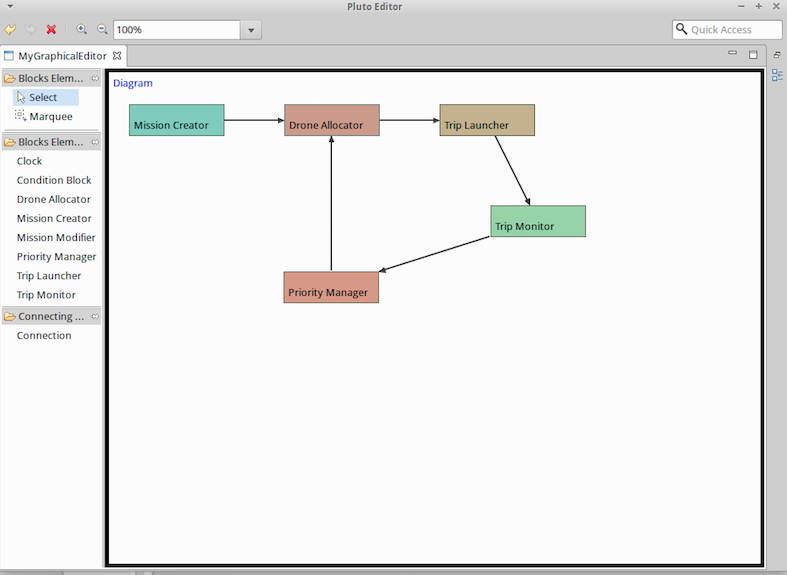
\includegraphics[width=\linewidth,height=7cm]{pictures/secondStep.png}
  \caption{Solution of the second step with Priority Manager}
  \label{fig:secondStepPriority}
\end{figure}

Then to add the Delay feature in the diagram the user needs to do the same thing with the Clock block, that provides the feature to wait for an amount of time, set in the delay attribute of a Trip. This block is taking as input the mission provided by the Trip Monitor and the by the Mission Creator then, after the delay time has passed, gives the mission to the DroneAllocator block, as shown in figure \ref{fig:secondStepClock}.

This is a useful step to compute, because the user learns how to use the connection element, that is a very important feature in the Pluto framework, and also the Priority Manager and Clock blocks.

\begin{figure}[htb]
  \centering
  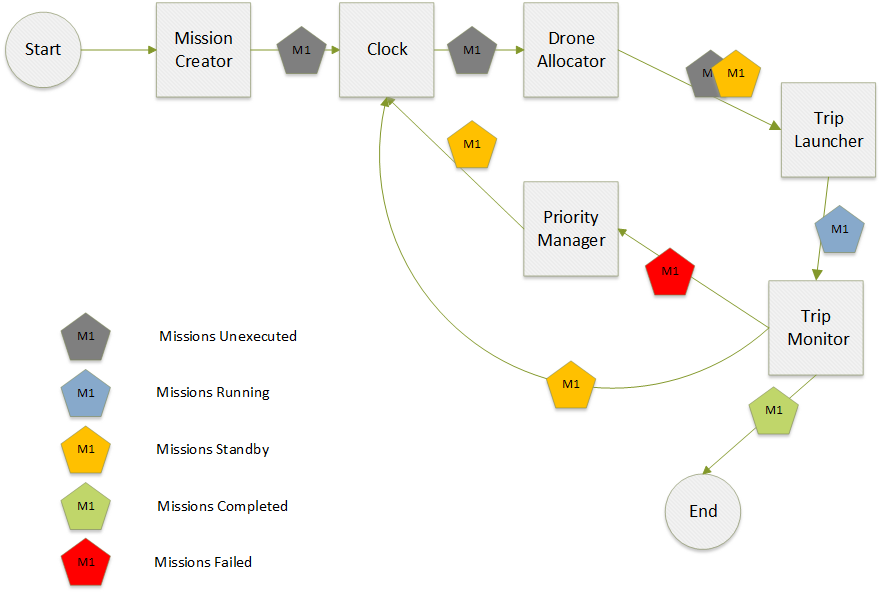
\includegraphics[width=\linewidth,height=7cm]{pictures/secondStepClock.png}
  \caption{Solution of the second step with Clock block}
  \label{fig:secondStepClock}
\end{figure}

\newpage


For the third step, the user has to implement the feature of the Timer Monitor block without using it.
So, he has to use the Mission Modifier block, through which he can insert his code in the application, and put it between the Trip Launcher and  Trip Monitor blocks, as shown in figure \ref{fig:thirdStep}.

This is a very useful step to compute, because the user learns how to use Mission Modifier block, which is the most important feature of the Pluto Editor, because it allows the programmer to insert his custom code to characterize the application.

\begin{figure}[H]
  \centering
  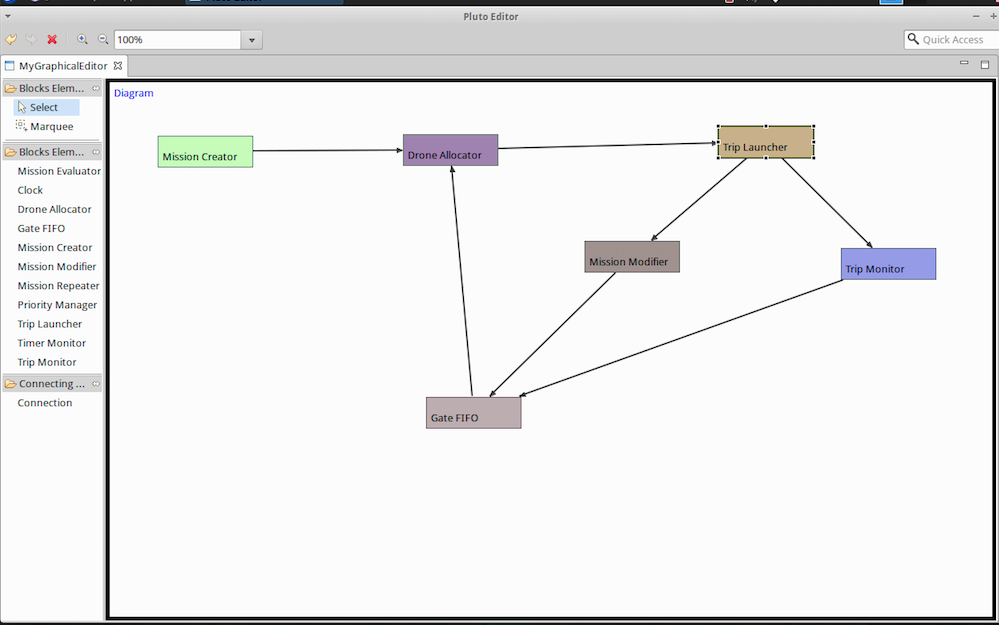
\includegraphics[width=\linewidth, height=8cm]{pictures/thirdStep.png}
  \caption{Solution of the third step}
  \label{fig:thirdStep}
\end{figure}

\subsubsection{Second Exercise}

The main purpose of this exercise is to underline possible issues in the code generated with the Pluto Graphical Editor. We must be sure that all the functionality described by the diagram are enabled in the generated code and that the missions execution will run smooth as the user expects. Any lack in the user experience may compromise the usability of the entire application, so it is important to evaluate the User Interface too. In this way, we check if the visual disposition of the graphics elements is appropriate.
The first step asks every user to create and run the same kind of missions, as described in the following list:

\begin{itemize}
\item Mission 1
	\subitem Trip A -> Action: Take Photo
    \subitem Trip B -> Action: Take Photo
    \subitem Trip C -> Action: Take Photo
\item Mission 2
	\subitem Trip A -> Action: Measure
    \subitem Trip B -> Action: Measure
\item Mission 3
	\subitem Trip A -> Action: Pick Item
    \subitem Trip B -> Action: Release Item
    \subitem Trip C -> Action: Take Photo
    \subitem Trip D -> Action: Measure
\end{itemize}

The location in the map of the Trips was not important while testing, so the tester could decide any place.
In the second step the users were asked to open the Monitor Page and to start the missions following their execution using the provided table and console.
The third step of the exercise consists in calling back the Drone with an RTL command.


\subsection{Evaluation metrics}\label{metrics}

To concretely evaluate the usability of the Pluto programming framework we defined the following metrics, which we applied for both exercises:

\begin{itemize}
\item {Number of people who correctly solved the first part of the exercise}
\item {Number of people who correctly solved the first and second parts of the exercise}
\item {Number of people who correctly solved the whole exercise}
\item {Mean time for the resolution of the first part of the exercise}
\item {Mean time for the resolution of the second part of the exercise}
\item {Mean time for the resolution of the third part of the exercise}
\item {Mean time for the resolution of the whole exercise}
\item {Number of people who solved the whole exercise, but in a wrong way}
\item {Number of people who could not solve the exercise at all}
\end{itemize}

Through metrics 1,2 and 3 we can understand which parts of the exercises are not clear for the user and/or too difficult to implement. 
Through metrics 4,5,6 and 7 we can understand, once the user has understood how to implement each feature, how much is difficult to solve each part of the exercises by measuring the time required to solve each step.
Through metrics 8 and 9, finally, we can understand how easy is to confuse the specifications and how many people couldn't solve any step of the exercises.


\subsection{Baseline}

We want to demonstrate the effective usefulness of the Pluto programming framework, so we decide to compare its features with the API of the Crazyflie Nano-quadcopter, which was described in section \ref{crazyflie}.

Actually, the crazyflie is the drone we chose to use for our applications case study, and we want to demonstrate that, without Pluto and using only the Crazyflie API would be very difficult to build the same kind of applications.

So we decide to propose another exercise to our users, but this time they can use only the Crazyflie API and they have a limited amount of time.

The Crazyflie API is written in Python, so we address to people who knows Python language features.

The exercise consists in make the drone moving from a point A to a point B on a map, performing a single Trip.

It may seem easy, but it can can take a long time to fully understand and apply the API in the correct way.


\subsection{User Survey}\label{survey}

Since we want to evaluate the usability of Pluto, we propose a survey, partly showed in figure \ref{fig:survey}, to the users, in order to understand how easy it is to use and which modifications should be applied to improve the user experience.

\begin{figure}[H]
  \centering
  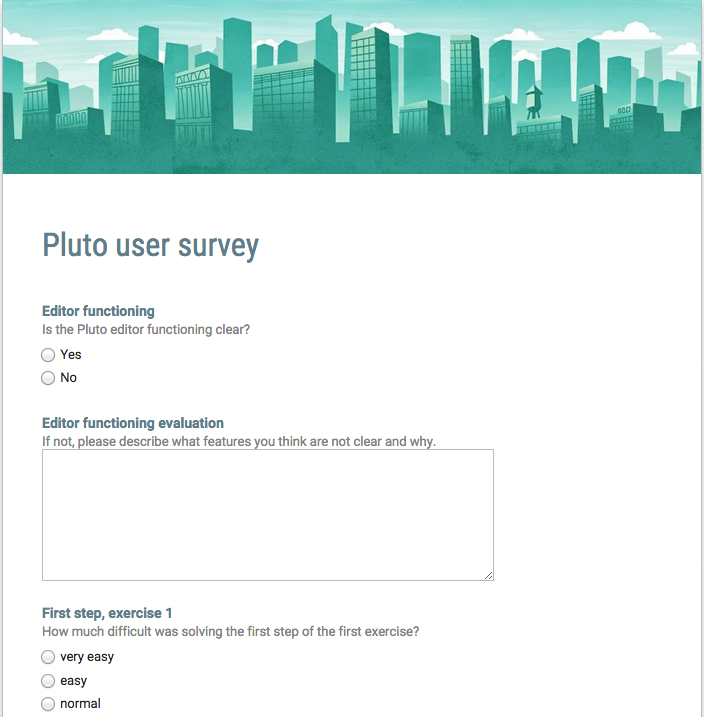
\includegraphics[width=\linewidth]{pictures/survey.png}
  \caption{Pluto user survey}
  \label{fig:survey}
\end{figure}

We ask users to tell us how easy was the development of the various steps of the exercises, and to provide us with a feedback on the usability of the editor and the main application underlining any problems found.
We also ask for suggestions to improve the usability of Pluto.

The survey can be found following this link:

\url{https://docs.google.com/forms/d/1b_52e7VLuns6AH1jiT3TeIRZ_KPRTLJYJe9ckrJanWY/viewform?usp=send_form}


Actually, this survey gives us very useful information about the Pluto framework. We can understand how "usable" it is and which modifications should be performed to improve the user's experience, also thanks to the visualization of the answers in a graphical way, shown in the next section, the \ref{surveyResult}.
Through the questions on the exercises development we can understand how difficult it is to create, modify,customize and execute a particular application, validating "on field" the use of the various blocks, especially the Mission Modifier, and the usability of the user interface.

\subsection{Final Results}\label{surveyResult}

Thanks to the combination of the answers to the user survey of section \ref{survey} and the numeric data collected according to the metrics defined in section \ref{metrics}, in this section we can show the results of the Pluto evaluation.
We make use of graphical representation in order to make the results clearer and easily understandable by everyone.
The metrics data are put into a table, while the results of the user survey are presented with graphics.

%qui vanno i dati delle nostre metriche, in una tabella

%qui vanno i grafici a torta che crea google survey

%qui un nostro commento sui risultati


\newpage

\section{Performance evaluation}\label{performance}

In order to strengthen the evaluation of Pluto, after the user study, described in Section \ref{usability}, we evaluated some qualitative metrics. These metrics are divided in two main types: software metrics and hardware consumption metrics. The former let us know the complexity of our software, on the other hand, the latter are useful to underline possible issues at run-time such as thread deadlock or a too high memory consumption.
Since our framework is composed by two main components, we decided to split this evaluation in two parts: this means that each kind of evaluation was performed on Pluto Graphical Editor first and then on Pluto Main Application.
To measure these parameters we used a very useful tool called VisualVM, shown in figure \ref{fig:visualVM}. 

\begin{figure}[H]
  \centering
  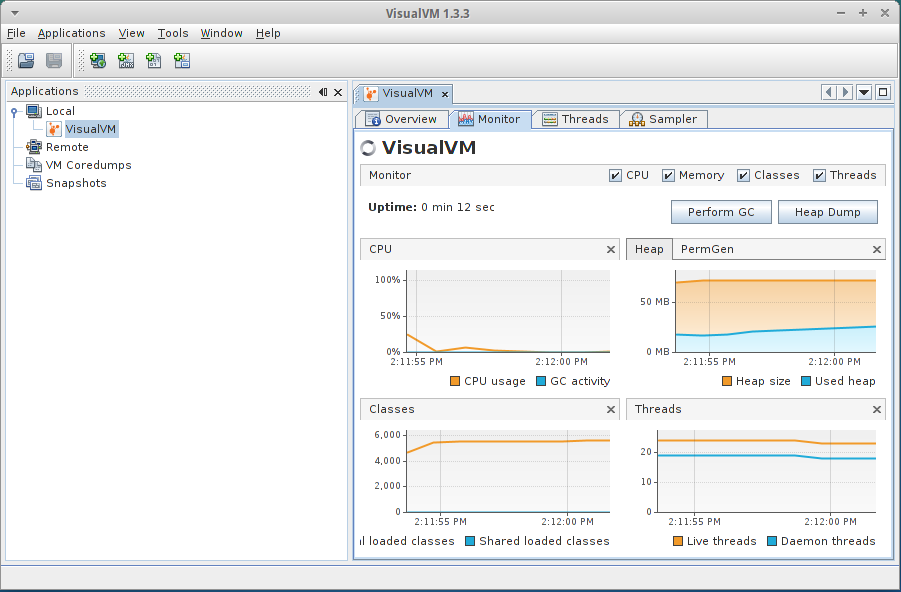
\includegraphics[width=\linewidth]{pictures/visualVM.png}
  \caption{VisualVM interface}
  \label{fig:visualVM}
\end{figure}

It let the user have a global monitoring of the running Java application in your local Java Virtual Machine, at run-time. Furthermore, it has a useful feature that records the profiling of an application in a dump file so that the user can compare different dump files concerning different application sessions.
Then, in the Result section \ref{metricsResult}, we describe the outcome of the tests for Pluto Graphical Editor and Pluto Main Application separately.

\subsection{Software Metrics}

The software metrics let us understand the complexity of the software, we decided to record these parameters for each component of Pluto Framework:

\begin{itemize}
\item Lines Of Code (LOC)
\item Number of classes attributes
\item Number of methods
\item Number of methods calls
\item ...
\end{itemize}

\subsection{Hardware Consumption}

The hardware metrics are those parameters measured at run-time, during the execution of the two software, to check if it generates any performance issues, because it could require too much resources to run smooth. These metrics are:

\begin{itemize}
\item CPU Load
\item Memory Consumption
\item Threads Generated
\item Threads Zombies (not terminated)
\item ...
\end{itemize}

The profiling of the application were done on a machine with these specs:

\begin{itemize}
\item CPU: Intel i7 2640
\item RAM: 4GB
\item VGA: Nvidia GeForce 610M
\item SSD: Kingston 120GB
\item OS: Xubuntu 14.04
\end{itemize}

Concerning the Pluto Graphical Editor, we measured those parameters while creating a lot of blocks and a very complex web of connections, shown in figure \ref{fig:stressDiagram} and then we observed the stress level while generating the source code of the Main Application from that drawing. We concentrated the evaluation on two parameters: the number of blocks and the number of connections. Firstly we fixed the former and we incremented the latter by a step of 5. Then we did the same operation fixing the number of connection and raising the number of blocks.

\begin{figure}[H]
  \centering
  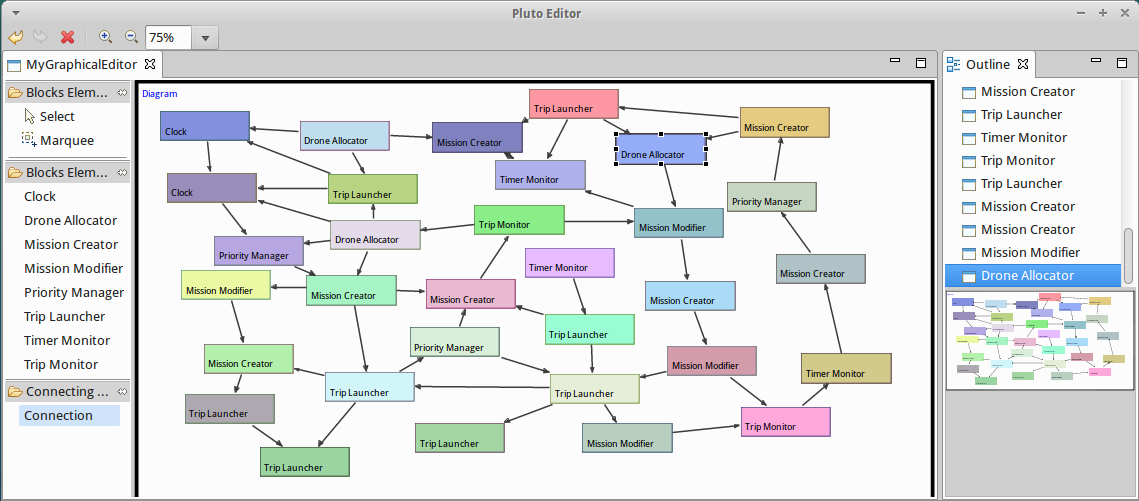
\includegraphics[width=\linewidth]{pictures/stressDiagram.png}
  \caption{Very Complex Diagram Example}
  \label{fig:stressDiagram}
\end{figure}

Furthermore, we evaluated the same metrics concerning the Main Application. We decided to focus this evaluation varying 3 important parameters: the number of Mission, the number of Trips related to a single Mission and the number of available Drones. We started fixing two of these parameters and raised the third step by step. Then we did again this procedure fixing another couple of parameters and varying the left one. In this way, we could evaluate the performance of the Main Application in an accurate way and the result are shown in next section \ref{metricsResult}.

\subsection{Result}
\label{metricsResult}

For software metrics there will be a table with 2 column and each row will be a metric: LOC, classes, ... The 2 columns are Editor and Main app.
\\
For the Performance part of the Editor there will be 2 graph, one with Connecton fixed and number of block raising up, the second is inverted. on X there will be the variable parameter and on Y the metrics: cpu, memory,...
For the performance part of the Main App, there will be 3 graphs: one with Mission and Trip fixed, then Drones will raise by a step of 5 starting from 1. On the X coord there will be Drones, on the Y coord there will be the metrics: cpu consume, memory usage, threads allocated, each line with a different color.
Then the same thing with Mission free, and then with Trip free.




\chapter{Conclusions and future works}
\label{cap7}

In this final Chapter we recap the structure of the whole document and the development phases of the Pluto programming framework.
We also show the limits of Pluto and the possible future works thanks to which these limits could be overcome.

\section{Conclusions}

We have developed the Pluto programming framework, a system which allows to build nano-drones applications for indoor contexts, simply by graphically connecting blocks.

In this document we have fully described the development process of Pluto and the context surrounding our work:
\\

In Chapter \ref{cap1} we have given the general context and the general goals of the work together with a brief description of the Pluto development process.
\\

In Chapter~\ref{cap2} we have described the three main existing approaches for drone programming, also proposing existing examples for each one of them.
We have shown that no one of these approaches is suitable for our requirements, since we needed the concepts of \textit{Mission} and \textit{Trip}.
A Mission is a list of sensing tasks to be performed sequentially and a Trip is a movement from a point A to a point B in the environment to perform an Action.
We have also described the dataflow programming method, providing two existing examples of it.
Also in this case, we have shown that we needed a different approach, since we needed to use only a group of basic features for our work, while the existing solutions were too general and contained a lot of complex components.
\\

Chapter~\ref{cap3} is focused on the problems stemming from the indoor context and on the requirements deriving from it.
Starting from a motivating example application, in order to better explain the requirements and problems deriving from our work, we have shown the implementation problems deriving from using a Team-level approach for our system, also proposing the solutions to fix them.
Finally we have shown the technological limitations affecting our system, such as the indoor localization and nano-drone batteries problems.
\\

In Chapter~\ref{cap4} we have presented our solution for the research problems described in Chapter ~\ref{cap3}, the Pluto programming framework.
We have presented our programming model, that is to say the main entities and the relationships between them.
We have described the functionality of the blocks of the Pluto Graphical Editor, that are the basic elements that the programmer can connect to graphically build an application.
We also have described in details the two components of the Pluto framework:
the Graphical Editor, that is used by the programmer to graphically build an application and the Main Application, that is used by the final user to specify the sensing tasks to be performed.
We have describe the navigation system, that is the conjunction point between the Main Application and the drones team.
We finally have shown all the steps performed to arrive to the final system, showing all the previously implemented solutions which, once refined, brought us to the development of the Pluto programming framework.
\\

In Chapter~\ref{cap5} we have shown how the designed choices have been implemented technically, describing all the software and tools we used for the development of Pluto programming framework.
We have described:
The GEF framework, which we have used to implement the Pluto Graphical Editor.
The code generation process that creates a Java application from the graph built with the Pluto Graphical Editor.
The Object-Oriented programming model of the Pluto framework.
The runtime features of Pluto: the parallel architecture and the management of all the needed threads.
The SWING tool, which we have used to develop the Pluto Main Application.
The Crazyflie nano-quadcopter, which we have used to perform the sensing tasks of our prototype applications.
\\

In Chapter~\ref{cap6} we have described four already existing applications and three case study, and we have discussed on whether they can be developed or not with Pluto. 
We have proposed two exercises to real testers, in order to test "on the field" the effective usability of Pluto:
the first one deals with the Graphical Editor, the second one with the Main Application.
Then we have proposed a third exercise, in which we ask the users to directly use the API of the Crazyflie nano-quadcopter, shown in Section \ref{crazyflie}, to make it move from a point A to a point B.
We have also proposed a survey to the users, in order to have opinions on the framework and possibly to improve it with the suggestions of the testers.
We also have measured the software and hardware consumption metrics required by Pluto, in order to evaluate the effective impact of Pluto on an ordinary computing machine.

\newpage

\section{Pluto limits and future works}

In this Section we show the limits of the Pluto programming framework.

There are two type of limits:
the limits in the implementation can possibly be overcome by modifying the source code and/or adding new features, or changing the whole model of the system.
The technological limits cannot be overcome in the present, and only research and studies can find a way to improve or find new technologies which would solve these problems.


The PURSUE application, described in Section \ref{PURSUE}, put in evidence the Pluto main limitation: the immediate execution of actions in response to instantaneous events.

As already explained in chapter \ref{cap4}, the Pluto system allows the drones to perform their actions only at the end of the Trip, that is a movement from a point A to a point B in the environment.
For example, if the Drone has to take a picture in a specific location, it flies from the ground station to that location and then it takes the picture.

There is no way to actively perform actions reacting on events:
so, as already explained, this is the problem of the PURSUE application, which requires to actively follow a moving object when it enters in the camera range.

This is an hint for the future expansion of Pluto, in order to manage also this kind of applications.
\\

As already explained in chapter \ref{cap3}, the actuation in indoor contexts is tricky because of the localization problem.
We showed some IPS methods, but still they are not as efficient and standardized as GPS.
They introduce latency in the localization mechanism and their precision is lowered by physical obstacles, roofs and ceilings.
\\

In this direction, research and future studies will certainly find a better indoor localization method, and Pluto will take advantage from it, since it has an architecture that is decoupled from the particular localization method.
So, when this new method will be implemented, it will be easily integrated with Pluto.
This is an important missing feature, since the actuation tasks performed by the drones completely relies and depends on a localization base:
in order to send a drone in a specific location to take a picture there is need of a method that precisely indicates that location.
\\

Research and future studies will also find a way to improve the capacity of the nano-drones batteries. 
Nowadays their duration is approximately of 7 minutes, with a recharge time of 20 minutes.
This is a great limitation, because the programmer is forced to develop applications where the sensing tasks must be performed within this limited amount of time.
\\
\\
\\

Finding a solution to the limitation of the instantaneous actuation, together with new technological discoveries that will improve the drones battery duration and find a good and stable indoor localization method, can greatly enrich the Pluto programming framework.
\\




\addcontentsline{toc}{chapter}{Bibliography}
\bibliographystyle{IEEEtran}
\bibliography{bib}{}

%\appendix
%
%\pagestyle{plain} 
%\renewcommand{\chaptermark}[1]{\markboth{\appendixname\ \thechapter.\ #1}{}} 
%\renewcommand{\sectionmark}[1]{\markright{\thesection.\ #1}}         
%\fancyhead[LE,RO]{\bfseries\thepage}    
%                                        
%\fancyhead[RE]{\bfseries\leftmark}    
%\fancyhead[LO]{\bfseries\rightmark}     
%\renewcommand{\headrulewidth}{0.3pt}

%\chapter{User survey}\label{appendixA}

\textbf{Editor functioning}
\\

Is the Pluto editor functioning clear?

 
\begin{itemize}
\item{Yes}
\item{No}
\end{itemize}


\textbf{Editor functioning evaluation}
\\

If not, please describe what features you think are not clear and why.
\\


\textbf{First step, exercise 1}
\\

How much difficult was solving the first step of the first exercise?


\begin{itemize}
\item{very easy}
\item{easy}
\item{normal}
\item{hard}
\item{very hard}
\item{not solved}

\end{itemize}


\textbf{First step evaluation, exercise 1}
\\

If you didn't solve the first step, or you find it hard or very hard, please explain why.
\\


\textbf{Second step, exercise 1}
\\

How much difficult was solving the second step of the first exercise?


\begin{itemize}
\item{very easy}
\item{easy}
\item{normal}
\item{hard}
\item{very hard}
\item{not solved}

\end{itemize}
 

\textbf{Second step evaluation, exercise 1}
\\

If you didn't solve the second step, or you find it hard or very hard, please explain why.
\\

\textbf{Third step, exercise 1}
\\

How much difficult was solving the Third step of the first exercise?


\begin{itemize}
\item{very easy}
\item{easy}
\item{normal}
\item{hard}
\item{very hard}
\item{not solved}

\end{itemize}


\textbf{Third step evaluation, exercise 1}
\\

If you didn't solve the third step, or you find it hard or very hard, please explain why.
\\ 

\textbf{Editor interface}
\\

Define the usability of the Pluto editor interface.


\begin{itemize}
\item{easily usable}
\item{normal}
\item{hard to use}
\item{obscure}

\end{itemize}

\textbf{Editor interface evaluation}
\\

If you answer is 'hard to use' or 'obscure', please explain what features are tricky and why.
\\ 

\textbf{Code generation}
\\

Is the code generation step easy to perform?


\begin{itemize}
\item{easy}
\item{normal}
\item{hard}

\end{itemize}

\textbf{Code generation evaluation}
\\

If you answer is 'hard', please explain what is not clear to you and why.
\\ 

\textbf{Editor suggestions}
\\

Please write here any comment/suggestions to improve Pluto Editor.
\\ 

\textbf{User application functioning}
\\

Is the Pluto user application functioning clear?


\begin{itemize}
\item{Yes}
\item{No}
\end{itemize}

\textbf{User application functioning evaluation}
\\

If not, please explain what features you think are not clear.
\\ 

\textbf{First step, exercise 2}
\\

How much difficult was solving the first step of the second exercise?


\begin{itemize}
\item{very easy}
\item{easy}
\item{normal}
\item{hard}
\item{very hard}
\item{not solved}

\end{itemize}

\textbf{First step evaluation, exercise 2}
\\

If you didn't solve the first step, or you find it hard or very hard, please explain why.
\\ 

\textbf{Second step, exercise 2}
\\

How much difficult was solving the second step of the second exercise?
 

\begin{itemize}
\item{very easy}
\item{easy}
\item{normal}
\item{hard}
\item{very hard}
\item{not solved}

\end{itemize}

\textbf{Second step evaluation, exercise 2}
\\

If you didn't solve the second step, or you find it hard or very hard, please explain why.
\\ 

\textbf{Third step, exercise 2}
\\

How much difficult was solving the third step of the second exercise?


\begin{itemize}
\item{very easy}
\item{easy}
\item{normal}
\item{hard}
\item{very hard}
\item{not solved}

\end{itemize}

\textbf{Third step evaluation, exercise 2}
\\

If you didn't solve the third step, or you find it hard or very hard, please explain why.
\\ 

\textbf{Missions page}
\\

How much difficult was to use the Missions Page of the Pluto user application?


\begin{itemize}
\item{very easy}
\item{easy}
\item{normal}
\item{hard}
\item{very hard}

\end{itemize}

\textbf{Missions page evaluation}
\\

If you find it hard or very hard, please explain why.
\\ 

\textbf{Trips page}
\\

How much difficult was to use the Trips Page of the Pluto user application?


\begin{itemize}
\item{very easy}
\item{easy}
\item{normal}
\item{hard}
\item{very hard}

\end{itemize}

\textbf{Trips page evaluation}
\\

If you find it hard or very hard, please explain why.
\\ 

\textbf{Monitor page}
\\

How much difficult was to use the Monitor Page of the Pluto user application?


\begin{itemize}
\item{very easy}
\item{easy}
\item{normal}
\item{hard}
\item{very hard}

\end{itemize}

\textbf{Monitor page evaluation}
\\

If you find it hard or very hard, please explain why.
\\ 

\textbf{User application suggestions}
\\

Please write here any comment/suggestions to improve Pluto user application.
\\ 


%\chapter{Implementation documentation}
\label{appB}

\noindent Documentazione della programmazione in piccolo dove si mostra la struttura ed eventualmente l'albero di Jackson.
%\chapter{Listing}
\label{appC}

\noindent Il listato (o solo parti rilevanti di questo, se risulta particolarmente esteso) con l'autodocumentazione relativa.
%\chapter{User manual}
\label{appD}

\noindent Manuale utente per l'utilizzo del sistema
%\chapter{Practical example}
\label{appE}

\noindent Un esempio di impiego del sistema realizzato.
%\chapter{Datasheet}
\label{appF}

\noindent Eventuali Datasheet di riferimento.

\end{document}